
%使用xelatex编译
%版权所有,翻版必究
%本文件由程序自动生成,任何修改将被覆盖
%2019 年 01 月 09 日




%主文档



\documentclass[12pt,hyperref,UTF8]{ctexbook}%使用大号字体

%解决新版latex一些BUG
\let\counterwithout\relax
\let\counterwithin\relax

%@P143
\usepackage{xcolor}        %导入包xcolor
\usepackage[
a4paper ,
left=2.0cm,                %靠近装订线的边距
right=2.0cm,               %远离装订线的边距
top=2.0cm,
bottom=2.0cm,
headheight=1.3cm,
headsep=0.5cm,
marginparsep=0.1cm,
marginparwidth=0.1cm
]{geometry}                %导入包geometry

 %导入常用包
\usepackage{graphicx}
\usepackage{float}
\usepackage{amsmath}
\usepackage{cite}
\usepackage{caption}
\usepackage{titlesec}
\usepackage{chngcntr}
\usepackage{setspace}
\usepackage{tocbibind}  %设置目录
\usepackage{tocloft}
\usepackage{multicol}
\usepackage{listings}   %引入程序代码

%%常见符号
\usepackage{wasysym}    %
\usepackage{textcomp}   %
\usepackage{pifont}     %

\usepackage{color}
\definecolor{colorbackgroundthisproject}{rgb}{1,1,1} %页面背景颜色
\definecolor{colortextthisproject}{rgb}{0,0,0}       %文字颜色
%设置页面颜色
\pagecolor{colorbackgroundthisproject}
%设置字体颜色
\color{colortextthisproject}

\usepackage{xhfill}
%\usepackage{times} do not use this pack ...

\usepackage{placeins}

%设置输出pdf格式
\usepackage[
    colorlinks=true ,
    %bookmarks=true,
    %bookmarksopen=false,
    %pdfpagemode=FullScreen,
    %pdfstartview=Fit,
    bookmarksnumbered=true,
    pdftitle={Qml} ,       %标题
    pdfauthor={Qml} ,      %作者
    pdfsubject={Qml} ,     %主题
    pdfkeywords={Qml} ,    %关键字
    linkcolor=colortextthisproject ,
    anchorcolor=colortextthisproject ,
    citecolor=colortextthisproject ,
    urlcolor=colortextthisproject
]{hyperref}

\usepackage{fontspec}
\definecolor{sourcegrayone}{rgb}{0.95,0.95,0.96}  %源代码背景颜色
\newfontfamily\sourcefontone{Consolas}            %源代码字体
\newfontfamily\sourcefontthree{DejaVu Sans Mono}  %源代码字体
%sudo apt-get install ttf-mscorefonts-installer   %linux安装字体
\newfontfamily\sourcefonttwo{Times New Roman}     %正文特殊符号字体
\renewcommand\lstlistingname{程序}
%源代码默认样式
\lstset{
language=C,
breaklines=true,
basicstyle=     \scriptsize\sourcefontthree        , %设置字号,字体
stringstyle=    \scriptsize\sourcefontthree        , %设置字号,字体
keywordstyle=   \scriptsize\sourcefontthree        , %设置字号,字体
commentstyle=   \scriptsize\sourcefontthree        , %设置字号,字体
identifierstyle=\scriptsize\sourcefontthree        , %设置字号,字体
numbers=left,
numberstyle=    \scriptsize\slshape\sourcefontone  , %设置字号,字体
frame=single,
backgroundcolor=\color{sourcegrayone},
showstringspaces=false
}

%设置item样式......
\usepackage{enumitem}
\setenumerate[1]{itemsep=0pt,partopsep=0pt,parsep=\parskip,topsep=5pt}
\setitemize[1]{itemsep=0pt,partopsep=0pt,parsep=\parskip,topsep=5pt}
\setdescription{itemsep=0pt,partopsep=0pt,parsep=\parskip,topsep=5pt}


%设置常量
\title{Qt Quick全面导引}                              %书籍名称
\author{Good Luck}                                   %作者名

%设置ctex
%@P135
\CTEXsetup[ number={ \arabic{chapter} } ]{chapter}
%\CTEXsetup[ number={ \arabic{section} } , name={第,节} ]{section}

\newenvironment{littlelongworld}
{ \\[0.25cm] }
{ \\[0.25cm] }

\newcommand\treeindexnumbernameone{目录树}
%\newcommand\theTreeIndexNumber{}
\newcounter{treeindexnumber}[chapter]
%\stepcounter{treeindexnumber}
%\refstepcounter{treeindexnumber}
\renewcommand\thetreeindexnumber{
    \thechapter.\arabic{treeindexnumber}
}

\newcommand\commandnumbernameone{命令行}
\newcounter{commandnumber}[chapter]
\renewcommand\thecommandnumber{
    \thechapter.\arabic{commandnumber}
}

%%%%%%%%%%%%%%%%%%%%%%%%%%%%
%解决目录字体重叠BUG
\makeatletter
\renewcommand{\numberline}[1]{%
\settowidth\@tempdimb{#1\hspace{0.5em}}%
\ifdim\@tempdima<\@tempdimb%
\@tempdima=\@tempdimb%
\fi%
\hb@xt@\@tempdima{\@cftbsnum #1\@cftasnum\hfil}\@cftasnumb}
\makeatother
%%%%%%%%%%%%%%%%%%%%%%%%%%%%

\begin{document}


\frontmatter
%%%%%%%%%%%%%%%%%%%%%%%%%%%%%%%%%%%%%%%%%%%%%%%%%%%%%%%%%%%%%%%%%%%%%%%%%%%%%

\pagestyle{empty}                 %关闭页眉页脚
\maketitle                        %生成封面
%%%%%%%%%%%%%%%%%%%%%%%%%%%%%%%%%%%%%%%%%%%%%%%%%%%%%%%%%%%%%%%%%%%%%%%%%%%%%

\cleardoublepage
\pagestyle{headings}              %开启页眉页脚
\pagenumbering{roman}             %重新开始页码编号
\setcounter{tocdepth}{4}          %设置目录深度
\setcounter{secnumdepth}{4}       %设置编号深度
\tableofcontents                  %生成目录
%%%%%%%%%%%%%%%%%%%%%%%%%%%%%%%%%%%%%%%%%%%%%%%%%%%%%%%%%%%%%%%%%%%%%%%%%%%%%

\mainmatter
%
%    arabic - 阿拉伯数字
%    roman  - 小写的罗马数字
%    Roman  - 大写的罗马数字
%    alph   - 小写的字符形式
%    Alph   - 大写的字符形式
%
\pagenumbering{arabic}           %重新开始页码编号
%%%%%%%%%%%%%%%%%%%%%%%%%%%%%%%%%%%%%%%%%%%%%%%%%%%%%%%%%%%%%%%%%%%%%%%%%%%%%

%使用xelatex编译
%版权所有,翻版必究
%本文件由程序自动生成,任何修改将被覆盖






\cleardoublepage                              %增加空白页
\setcounter{secnumdepth}{-2}                  %暂停编号,但加入目录
\chapter{
前言
}\label{c000020}
\setcounter{secnumdepth}{3}                   %恢复编号


%简单介绍Qt...
Qt往往被认为是一套跨平台的图形界面开发架构。
诚然,Qt对于图形界面支持的很好,并且,这一方面被越来越多的团队所接纳。
但Qt并不仅限于开发图形界面,它其实是一种更加通用的客户端开发架构。
Qt几乎提供了用于构建一个客户端所需的所有模块,包括但不限于
蓝牙模块、
串口模块、
音频模块、
网络模块、
多媒体模块、
数据库模块……

更加令用户愉悦的是,由于Qt本身是被广泛使用的开源产品,
用户可以轻松的享受到来自整个开源社区(其中包括整个C/C++社区)的加持。
也就是,
即使Qt本身并未提供一些方面的支持(或者Qt自身提供的支持无法满足要求),
用户也可以轻松的找到免费或付费的解决方案。
即使有些情况下用户无法找到解决麻烦的现成并有效的手段,
但至少通过社区,
用户可以获得一些走出困境的灵感。

%简单介绍QML+QtQuick...
随着新的硬件设备的广泛采用和开发者观念的变更。
完全采用C++这类静态计算机语言开发图形界面变得越来越笨手笨脚,
并且最终效果亦不佳,
很多由动态语言轻松可以达到的效果往往用静态计算机语言难以实现。
所幸的是,Qt一直没有停下前行的脚步。
Qml以及基于Qml的Qt Quick被引入和大力推广。
Qml本身被设计为一种简单而优雅的脚本语言,并且,
Qml天然支持一个JavaScript子集
\footnote{
主要是在Qml中禁用了JavaScript中this这个
语义模糊的关键字,并禁用JavaScript中的全局变量。
}。
用户可以安心的用C++做基础模块,
而利用Qt Quick将一切快速的组织起来。


Qt Quick比传统的Qt Widgets不仅仅更加有效利用CPU多核资源
(Qt Quick可以异步渲染)。
更令人高兴的是,Qt Quick完全是在显卡端完成渲染。
即使某些设备不支持显卡渲染,Qt自身也可以通过软件模拟达到效果。
这一切并不受限于某几个平台,而是几乎所有平台。
智能手机、个人电脑、嵌入式设备,它们都受到支持。
用户可以使用Qt Quick敏捷的构造出美观、高效、稳健并跨平台的一流产品。

Qt公司为用户提供了大量的辅助工具。
用这些工具,用户可以迅速的编写、测试、调试、部署、以及调优和美化。
除了Qt公司直接提供的工具外,
由于Qt的广泛使用,
很多第三方工具链也支持Qt。
虽然,到目前为止,
这些第三方支持主要是面向传统Qt C++。
但仅仅来自Qt自身的工具链对于Qt Quick的支持也不会令用户失望。


%简单介绍如何阅读本书...
本书是一本完整介绍Qt Quick的书。
通过本书,读者可以完整的掌握整个Qt Quick的全貌。
但限于篇幅和个人精力所限,一些细节可能被舍弃。

读者在阅读本书之前应当对于Qt C++、JavaScript和OpenGL具有一定了解,
并具备一定的图形学相关知识。
为了避免本书变成数千页的大部头,
本书并不会对上述细节多做解释。

基于Qt Qml的另一个模块是Qt 3D。
Qt 3D和Qt Quick是两个几乎不关联的模块,
虽然它们都基于Qt Qml。
本书并不介绍Qt 3D。

本书采用C++17标准编写,
Qt最低版本为Qt 5.12.0,
FFMPEG版本最低为4.1,
Boost版本为1.69.0,
如果读者在编译本书代码出现了问题,
请尝试查询当前开发环境是否正确。
本书只支持桌面Windows和桌面Linux,
这两个平台已经足够涵盖绝大多数读者,并能够完整诠释所有技术细节。
对于刚刚接触Qt Quick的读者,
一方面太多平台细节会成为干扰读者统揽全局的噪音;
另一方面对于一个具体的平台,
本书采用的一些技术特性可能不被支持
\footnote{
一些平台可能只支持有限的C++17标准和OpenGL特性,
另一方面在一些平台下FFMPEG也难以编译,
而且Qt自带的多媒体库在特定平台下如何部署也千差万别,
甚至有些平台可能根本不支持Qt 5.12.0及其后续版本而只支持一些老的Qt版本。
},
这些细节将极大拖慢本书的写作进度和涵盖的范围。
为了向读者展示一个全面的并且现代的Qt,本书不得不舍弃过多的平台适配而轻装上阵。

本书
第 \ref{c000010}章带领读者纵览整个Qt Quick,
对于Qt Quick不太熟悉的读者可能读起来有些吃力。
对于第 \ref{c000010}章,
初次阅读起来有些困难的地方直接跳过即可。

本书
第 \ref{c000011}章介绍Qt Qml基础语法以及Qt Quick基本元素,
第 \ref{c000012}章介绍如何使用C++扩展Qt Quick,
第 \ref{c000018}章介绍Qt Quick基础控件,
这三章是主干章节。

第 \ref{c000013}章介绍Qt Quick动画和状态机,
第 \ref{c000014}章介绍Qt Quick粒子系统,
第 \ref{c000015}章介绍一些常见特效,
第 \ref{c000017}章介绍Qt Quick的图文表模块,
第 \ref{c000019}章介绍Qt Quick的模型视图模块。
第 \ref{c000016}章本书介绍如何结合FFMPEG构建多媒体模块。
这些章节各有主题,读者根据需要选读即可。

\begin{lstlisting}[label=f000000, 
caption=GoodLuck,
title=\ \lstlistingname\ \thelstlisting
]
#include <iostream>

int main(int argc,char ** argv){
    std::cout << "Hellow World!" << std::endl;
    return 0;
}
\end{lstlisting}          %抄录环境

\begin{lstlisting}[label=f000001, 
caption=GoodLuck,
title=\ \lstlistingname\ \thelstlisting
]
#include <iostream>

int main(int argc,char ** argv){
    std::cout << "Hellow World!" << std::endl;
    return 0;
}
\end{lstlisting}          %抄录环境


















%使用xelatex编译
%版权所有,翻版必究
%本文件由程序自动生成,任何修改将被覆盖



     %前言

%使用xelatex编译
%版权所有,翻版必究
%本文件由程序自动生成,任何修改将被覆盖
%2019 年 01 月 09 日




%\FloatBarrier
\cleardoublepage
\chapter{
Qt Quick入门导引
}\label{c000010}





%......

%使用xelatex编译
%版权所有,翻版必究
%本文件由程序自动生成,任何修改将被覆盖





\section{
搭建开发环境
}\label{s100110}




%......


%使用XeLaTeX编译
%版权所有,翻版必究
%本文件由程序自动生成,任何修改将被覆盖
%2019 年 01 月 23 日




%

\FloatBarrier
\subsection{
在Windows平台下搭建开发环境
}\label{s000110}


\FloatBarrier
\subsubsection{
在Windows平台下安装Qt
}\label{ss000110}


读者可以到 \url{http://download.qt.io/archive/
}
下载最新的Qt运行环境。
然而,遗憾的是,从Qt 5.12.0开始从此网址下载的Windows平台下的Qt开发环境并不完整。
%介绍如何下载在线安装包...
读者不得不访问Qt官网 \url{https://www.qt.io
},
注册Qt帐号,然后按照流程下载在线安装包。
不得不说,这对初学者很不友好。
幸运的是,目前Qt网站有一个漏洞。读者可以直接访问
 \url{https://www.qt.io/download-thank-you
},点击“here”下载在线安装包。如\figurename\ \ref{p000000}。
%begin图片
\begin{figure}[htb] %浮动体 here and top ...
%there must use marginnote ...
\marginnote{\setlength\fboxsep{2pt}\fbox{\footnotesize{\kaishu\figurename\,}\footnotesize{\ref{p000000}}}}\centering %中心对齐
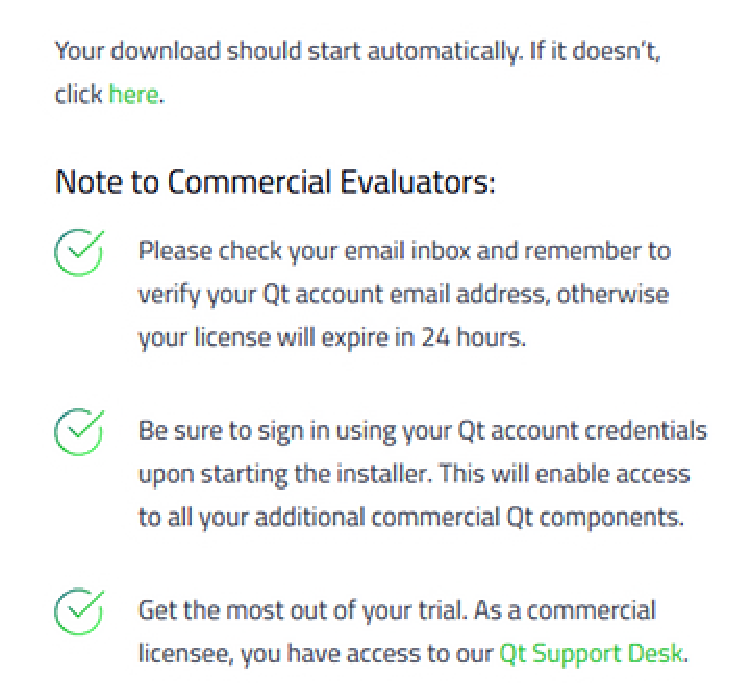
\includegraphics[width=8cm]{the_book_image/p000000.eps} %图片路径
\caption{Qt在线安装包下载路径} %标题
\label{p000000} %索引
\end{figure}
%end图片

以管理员身份运行在线安装包,
选择安装路径时请不要选择包含空格和中文字符的路径。
虽然现代开发环境对于空格和中文字符支持良好,
但是,很多第三方辅助工具未必支持空格和中文字符。
包括本书自带的辅助工具也不保证支持空格和中文。

在Windows平台下,建议读者选择安装“MSVC 2017 64\hspace{0.05em}\rule[0.7ex]{0.4em}{0.65pt}\hspace{0.05em}bit”或以上版
或者
“MinGW 7.3.0 64\hspace{0.05em}\rule[0.7ex]{0.4em}{0.65pt}\hspace{0.05em}bit”或以上版本。
Qt选择5.12.0或以上版本。
安装的时候最好选择安装“Sources”、“Qt Charts”、“Qt WebEngine”以及
“Qt Debug Information Files”这些模块。
在“Tools”选项下组好安装“CDB”以及对应的“MinGW”。
本书建议最小安装如\figurename\ \ref{p000001}。
%begin图片
\begin{figure}[htb] %浮动体 here and top ...
%there must use marginnote ...
\marginnote{\setlength\fboxsep{2pt}\fbox{\footnotesize{\kaishu\figurename\,}\footnotesize{\ref{p000001}}}}\centering %中心对齐
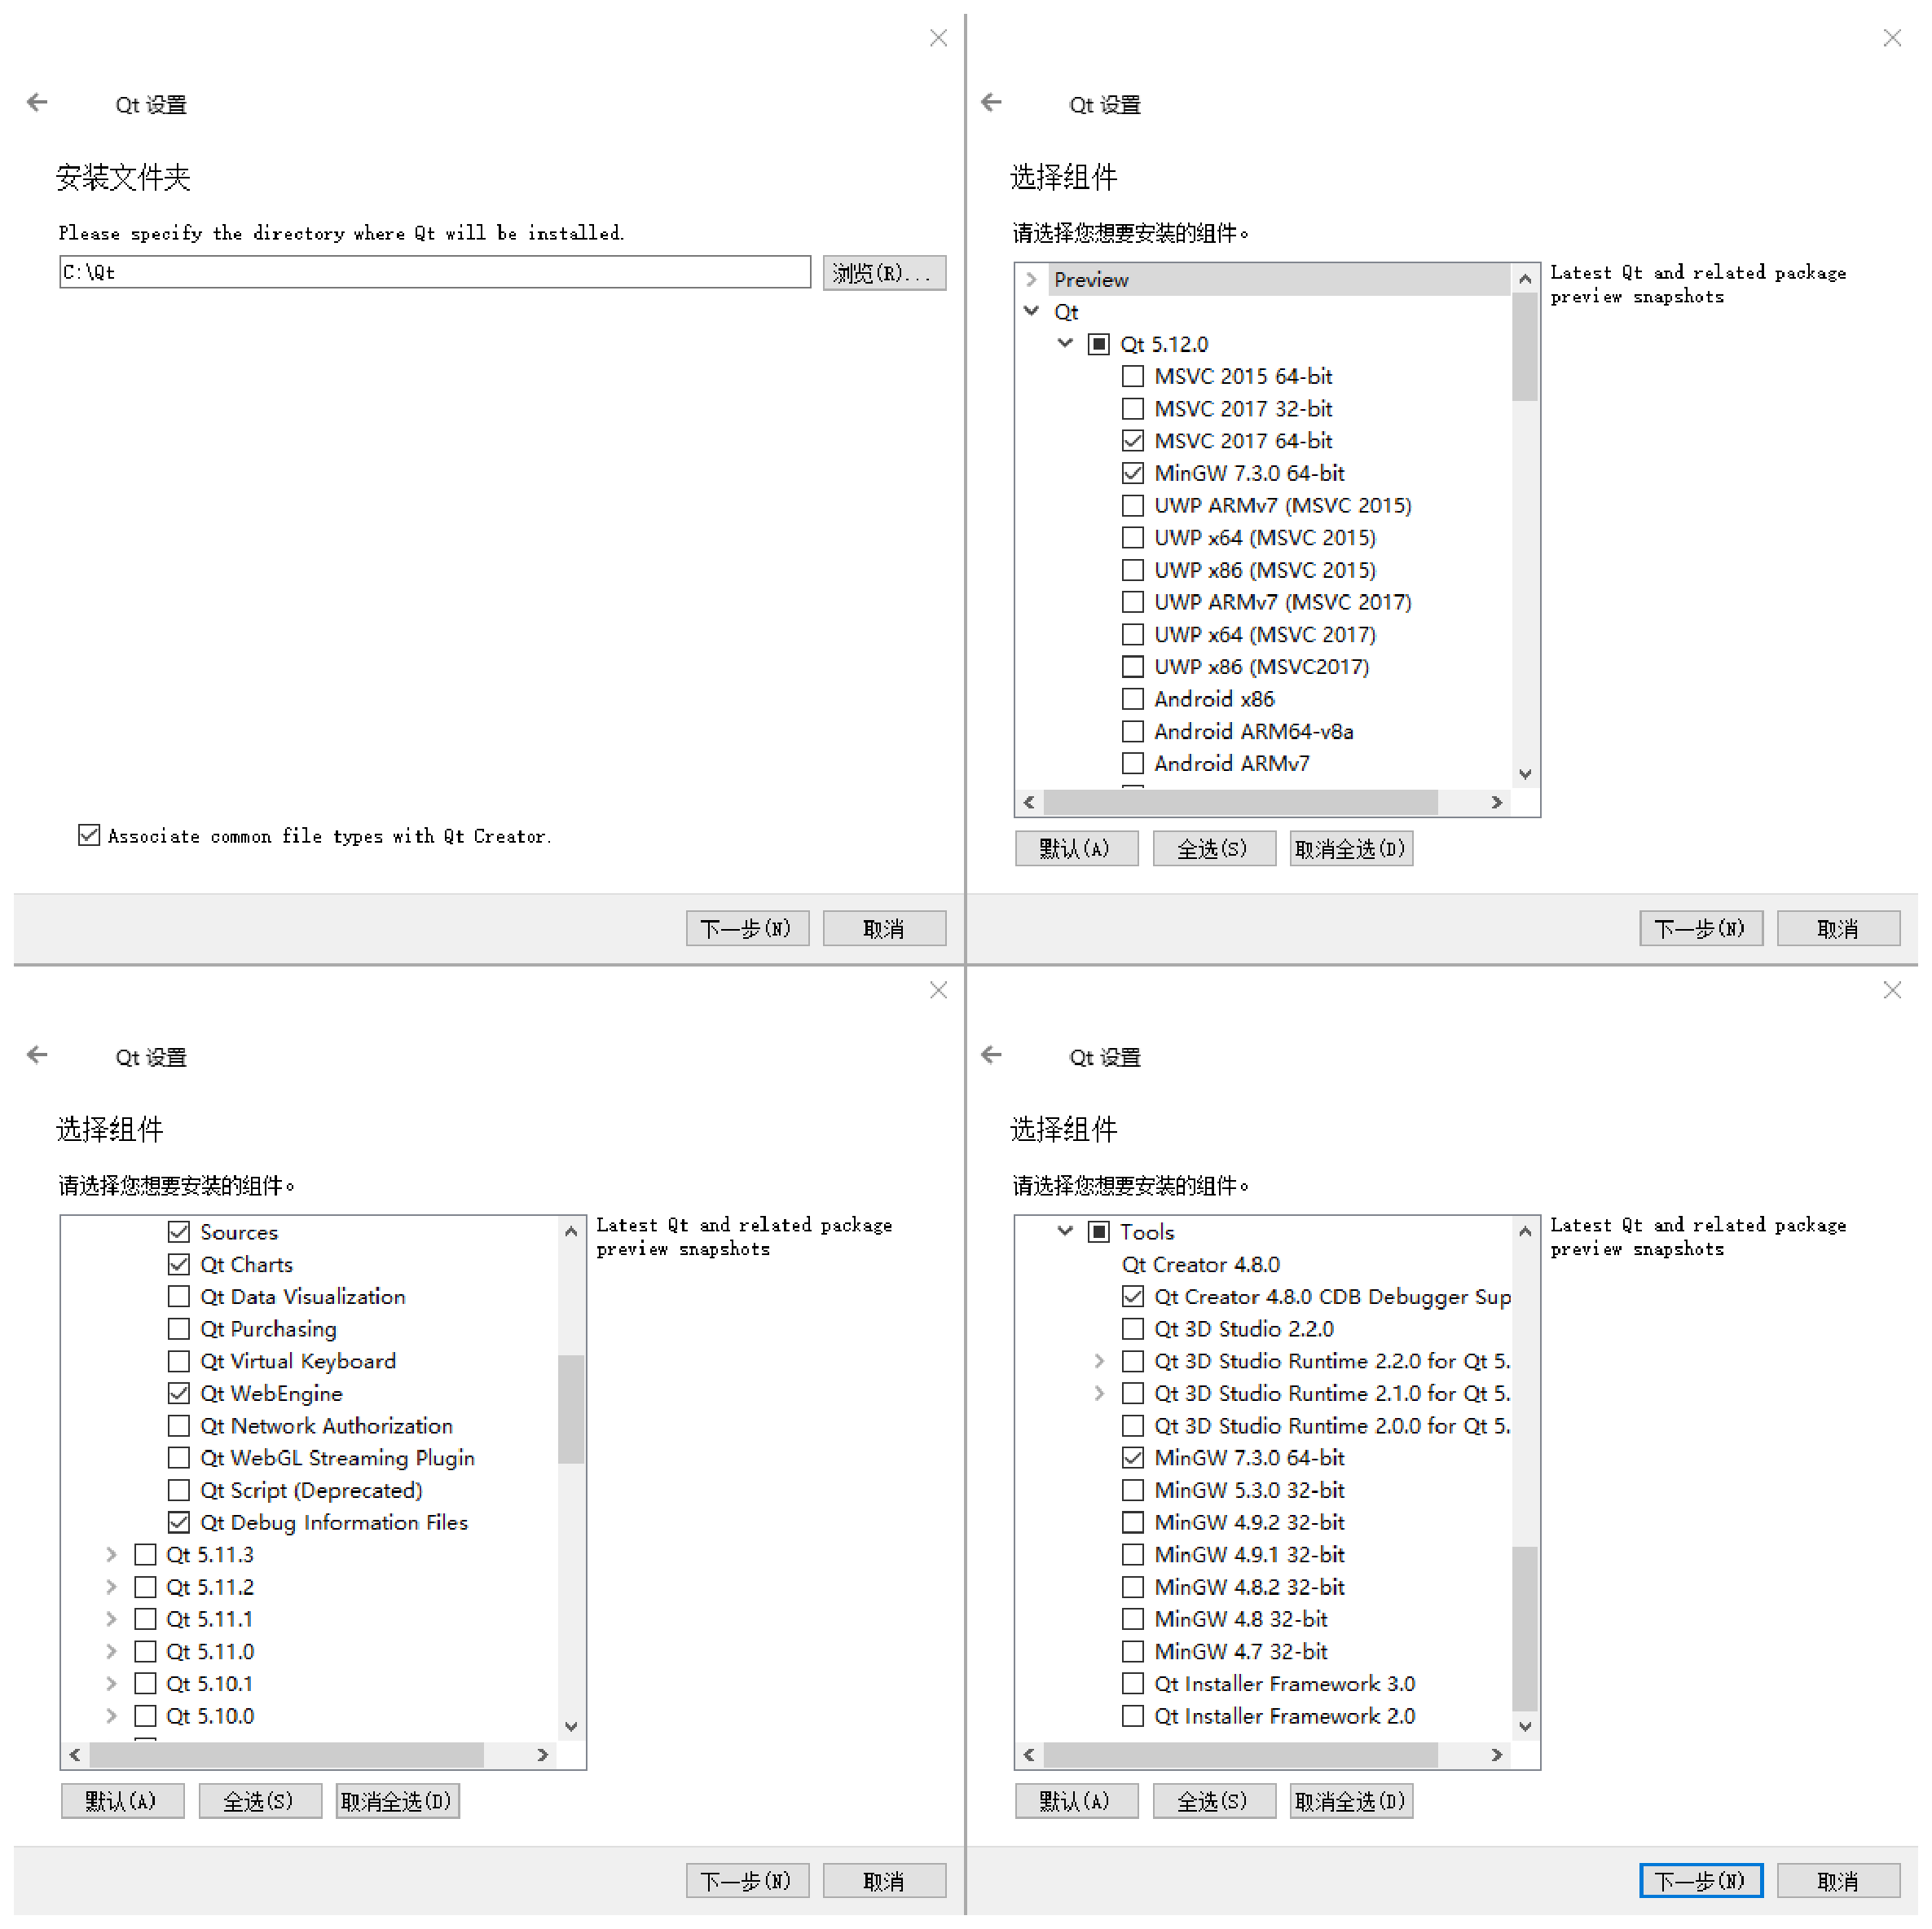
\includegraphics[width=0.95\textwidth]{the_book_image/p000001.eps} %图片路径
\caption{Qt在线安装建议安装组件} %标题
\label{p000001} %索引
\end{figure}
%end图片


\FloatBarrier
\subsubsection{
在Windows平台下安装Boost
}\label{ss000210}

读者需要到Boost官网 \url{https://www.boost.org/
}下载最新Boost稳定版。解压缩,将“boost”文件夹复制到Qt Include路径。

比如,
用户的Qt Include路径为:
\begin{littlelongworld}
C:\textbackslash{}Qt\textbackslash{}Qt5.12.0\textbackslash{}5.12.0\textbackslash{}msvc2017\underline{\hspace{0.5em}}64\textbackslash{}include
\end{littlelongworld}
\hspace*{\parindent}复制完boost之后,
应当存在路径:
\begin{littlelongworld}
C:\textbackslash{}Qt\textbackslash{}Qt5.12.0\textbackslash{}5.12.0\textbackslash{}msvc2017\underline{\hspace{0.5em}}64\textbackslash{}include\textbackslash{}boost
\end{littlelongworld}
\hspace*{\parindent}当然,读者也可以采用“mklink”建立链接代替拷贝。

如果读者使用的是Visual Studio自带的编译器,则需要使用“Visual Studio命令提示符”运
行\commandnumbernameone\ \ref{command000002s02}。
并将编译结果的“\raisebox{-0.35ex}{\sourcefonttwo{}*}.lib”文件拷贝到Qt根目录下的lib文件夹,
将“\raisebox{-0.35ex}{\sourcefonttwo{}*}.dll”文件拷贝到Qt根目录下的bin文件夹。

\renewcommand\thelstnumber{\ifnum\value{lstnumber}>3{\ }\else{\arabic{lstnumber}}\fi}
%\begin{spacing}{1.0}
%\FloatBarrier
\refstepcounter{commandnumber}\label{command000002s02}    %增加命令行编号
\begin{thebookfilesourceonecommand}[escapeinside={(*@}{@*)},
caption=GoodLuck,
title=\commandnumbernameone \thecommandnumber
]
cd /D < Boost源代码路径 >
bootstrap.bat
bjam --build-type=complete
     --toolset=< MSVC版本比如:msvc-14.1 >
     address-model=64
     link=shared
     runtime-link=shared
     threading=multi(*@\marginpar[\hfill\setlength\fboxsep{2pt}\fbox{\footnotesize{\kaishu\parbox{1em}{\setlength{\baselineskip}{2pt}\commandnumbernameone}}\footnotesize{\thecommandnumber}}]{\setlength\fboxsep{2pt}\fbox{\footnotesize{\kaishu\parbox{1em}{\setlength{\baselineskip}{2pt}\commandnumbernameone}}\footnotesize{\thecommandnumber}}}@*)\end{thebookfilesourceonecommand}          %抄录环境
\addtocounter{lstlisting}{-1}   %sub lstlisting counter ...
%\end{spacing}

\renewcommand\thelstnumber{\arabic{lstnumber}}

之后,读者需要根据编译输出更新“QtQmlBook/msvc\underline{\hspace{0.5em}}boost.pri”文件。
如\filesourcenumbernameone\ \ref{f000041}
所示:
%\begin{spacing}{1.0}
\refstepcounter{filesourcenumber}\label{f000041}    %增加源代码编号
\FloatBarrier                                  %强制完成浮动体布局
\begin{thebookfilesourceone}[escapeinside={(*@}{@*)},
caption=GoodLuck,
title=\filesourcenumbernameone \thefilesourcenumber
,numbers=none]
CONFIG(debug,debug|release){
    LIBS += "boost_atomic-vc141-mt-gd-x64-1_68.lib"
    ……
else{
    LIBS += "boost_atomic-vc141-mt-x64-1_68.lib"
    ……
}(*@\marginpar[\hfill\setlength\fboxsep{2pt}\fbox{\footnotesize{\kaishu\parbox{1em}{\setlength{\baselineskip}{2pt}\filesourcenumbernameone}}\footnotesize{\thefilesourcenumber}}]{\setlength\fboxsep{2pt}\fbox{\footnotesize{\kaishu\parbox{1em}{\setlength{\baselineskip}{2pt}\filesourcenumbernameone}}\footnotesize{\thefilesourcenumber}}}@*)\end{thebookfilesourceone}          %抄录环境
\addtocounter{lstlisting}{-1}   %sub lstlisting counter ...
%\end{spacing}


如果读者使用的是MinGW环境,则需要使用“MinGW命令提示符”运
行\commandnumbernameone\ \ref{command000002s01}。
并将编译结果的“\raisebox{-0.35ex}{\sourcefonttwo{}*}.a”文件拷贝到Qt根目录下的lib文件夹,
将“\raisebox{-0.35ex}{\sourcefonttwo{}*}.dll”文件拷贝到Qt根目录下的bin文件夹。

\renewcommand\thelstnumber{\ifnum\value{lstnumber}>3{\ }\else{\arabic{lstnumber}}\fi}
%\begin{spacing}{1.0}
%\FloatBarrier
\refstepcounter{commandnumber}\label{command000002s01}    %增加命令行编号
\begin{thebookfilesourceonecommand}[escapeinside={(*@}{@*)},
caption=GoodLuck,
title=\commandnumbernameone \thecommandnumber
]
cd /D < Boost源代码路径 >
bootstrap.bat
bjam --build-type=complete
     --toolset=gcc
     address-model=64
     link=shared
     runtime-link=shared
     threading=multi(*@\marginpar[\hfill\setlength\fboxsep{2pt}\fbox{\footnotesize{\kaishu\parbox{1em}{\setlength{\baselineskip}{2pt}\commandnumbernameone}}\footnotesize{\thecommandnumber}}]{\setlength\fboxsep{2pt}\fbox{\footnotesize{\kaishu\parbox{1em}{\setlength{\baselineskip}{2pt}\commandnumbernameone}}\footnotesize{\thecommandnumber}}}@*)\end{thebookfilesourceonecommand}          %抄录环境
\addtocounter{lstlisting}{-1}   %sub lstlisting counter ...
%\end{spacing}

\renewcommand\thelstnumber{\arabic{lstnumber}}

之后,读者需要根据编译输出更新“QtQmlBook/mingw\underline{\hspace{0.5em}}boost.pri”文件。
如\filesourcenumbernameone\ \ref{f000040}
所示:
%\begin{spacing}{1.0}
\refstepcounter{filesourcenumber}\label{f000040}    %增加源代码编号
\FloatBarrier                                  %强制完成浮动体布局
\begin{thebookfilesourceone}[escapeinside={(*@}{@*)},
caption=GoodLuck,
title=\filesourcenumbernameone \thefilesourcenumber
,numbers=none]
CONFIG(debug,debug|release){
    LIBS += "libboost_atomic-mgw73-mt-d-x64-1_68.dll"
    ……
}else{
    LIBS += "libboost_atomic-mgw73-mt-x64-1_68.dll"
    ……
}(*@\marginpar[\hfill\setlength\fboxsep{2pt}\fbox{\footnotesize{\kaishu\parbox{1em}{\setlength{\baselineskip}{2pt}\filesourcenumbernameone}}\footnotesize{\thefilesourcenumber}}]{\setlength\fboxsep{2pt}\fbox{\footnotesize{\kaishu\parbox{1em}{\setlength{\baselineskip}{2pt}\filesourcenumbernameone}}\footnotesize{\thefilesourcenumber}}}@*)\end{thebookfilesourceone}          %抄录环境
\addtocounter{lstlisting}{-1}   %sub lstlisting counter ...
%\end{spacing}


\FloatBarrier
\subsubsection{
在Windows平台下MinGW配置jemalloc
}\label{ss000310}


%LD_PRELOAD
%由于Windows平台下不存在类似于Linux平台“LD_PRELOAD”这样可以动态
对于C{\sourcefonttwo{}+}{\sourcefonttwo{}+}来说,小对象的内存碎片问题向来很棘手。
一般而言,使用tcmalloc或jemalloc可以有效避免内存碎片问题。

在Linux平台或类似平台下,
可以使用“LD\underline{\hspace{0.5em}}PRELOAD”或类似的技术轻松的覆盖动态链接库中的函数。
因而,在Linux平台下,使用tcmalloc或jemalloc替换C库中的内存分配函数是简易的。

而在Windows平台下,
覆盖动态库中的函数相当复杂。
为了能够使得本书的示例代码不是玩具,
本书在Windows平台下使用jemalloc克服小对象内存碎片。

当使用MSVC编译器的时候,本书直接嵌入jemalloc源代码,
因而读者不必特别操心。
但是,当在Windows下使用MinGW编译器时,
读者需要自己静态编译jemalloc\footnote{
如果读者使用MinGW 7.3 64 bit版本的编译器,
本书已经将对应版本的jemalloc编译好了,
读者不需要再次编译。
}。
并将编译结果放置到:
\begin{littlelongworld}
QtQmlBook\textbackslash{}sstd\underline{\hspace{0.5em}}library\textbackslash{}memory\textbackslash{}libs
\end{littlelongworld}
文件夹下。
并将文件重命名为“jemalloc\underline{\hspace{0.5em}}win64\underline{\hspace{0.5em}}mingw\underline{\hspace{0.5em}}730.a”。
如果读者实在无法静态编译jemalloc,
读者可以找到:
\begin{littlelongworld}
QtQmlBook\textbackslash{}sstd\underline{\hspace{0.5em}}library\textbackslash{}\underline{\hspace{0.5em}}sstd\underline{\hspace{0.5em}}library\underline{\hspace{0.5em}}memory.pri
\end{littlelongworld}
并将此文件内容清空\footnote{
注意不要删除这个文件,而只是删除此文件内容。
}。


















%使用XeLaTeX编译
%版权所有,翻版必究
%本文件由程序自动生成,任何修改将被覆盖
%2019 年 01 月 23 日




%使用xelatex编译
%版权所有,翻版必究
%本文件由程序自动生成,任何修改将被覆盖




%


\subsection{
在Linux平台下搭建开发环境
}\label{s000210}



\subsubsection{
在Linux平台下安装Qt
}\label{ss000410}





\subsubsection{
在Linux平台下安装Boost
}\label{ss000510}












%使用xelatex编译
%版权所有,翻版必究
%本文件由程序自动生成,任何修改将被覆盖























%使用xelatex编译
%版权所有,翻版必究
%本文件由程序自动生成,任何修改将被覆盖





%使用XeLaTeX编译
%版权所有,翻版必究
%本文件由程序自动生成,任何修改将被覆盖
%2019 年 01 月 23 日



%Gook Luck!

\FloatBarrier
\section{
qmake入门
}\label{s100310}


qmake类似于cmake,但qmake比cmake更加简洁清晰。
如果读者希望写一个跨平台的通用库的话,
或许cmake是比qmake更加优异的选择。
但读者明确是写一个特定的应用程序的话,
qmake就比cmake优秀的多。
qmake比cmake功能较少,
但从另一个角度,
qmake比cmake更加专注。
通过本节,
读者会发现只需要学习可怜的一点内容,
就可以使用qmake搭建出复杂的程序架构。
不过,本书毕竟是一门专门写Qt Quick的书,
不可能介绍qmake的每一个细节。

%%%%%%%%%%%%%%%%%%%%%%%%%%%%%%%%%%%%%%%%%%%%%%%%%%%%%%%%
\FloatBarrier
\subsection{
使用qmake构建Hellow World!
}\label{ss000610}

读者新建一个目录\footnote{
本书所有目录都要求不包含空格和中文,以后不再赘述。
},
在此文件夹下新建一个“hellow\underline{\hspace{0.5em}}world.pro”文件,输入文件内容如
\filesourcenumbernameone\ \ref{f000002}。
在此文件夹下建立“main.cpp”文件,输入内容如
\filesourcenumbernameone\ \ref{f000003}。

%\begin{spacing}{1.0}
\refstepcounter{filesourcenumber}\label{f000002}    %增加源代码编号
\FloatBarrier                                  %强制完成浮动体布局
\begin{thebookfilesourceone}[escapeinside={(*@}{@*)},
caption=GoodLuck,
title=\filesourcenumbernameone \thefilesourcenumber
]
QT -= gui
QT -= core

CONFIG += console

CONFIG(debug,debug|release){
    TARGET = hellow_word_debug
}else{
    TARGET = hellow_word
}

TEMPLATE = app

win32-msvc*{
    QMAKE_CXXFLAGS += /std:c++latest
}else{
    CONFIG += c++17
}

SOURCES += $$PWD/main.cpp
DESTDIR =  $$PWD

DEFINES *= NUMBER=1
DEFINES *= HELLOW=\\\"Hellow\\\"
DEFINES += QT_DEPRECATED_WARNINGS(*@\marginpar[\hfill\setlength\fboxsep{2pt}\fbox{\footnotesize{\kaishu\parbox{1em}{\setlength{\baselineskip}{2pt}\filesourcenumbernameone}}\footnotesize{\thefilesourcenumber}}]{\setlength\fboxsep{2pt}\fbox{\footnotesize{\kaishu\parbox{1em}{\setlength{\baselineskip}{2pt}\filesourcenumbernameone}}\footnotesize{\thefilesourcenumber}}}@*)\end{thebookfilesourceone}          %抄录环境
\addtocounter{lstlisting}{-1}   %sub lstlisting counter ...
%\end{spacing}

%\begin{spacing}{1.0}
\refstepcounter{filesourcenumber}\label{f000003}    %增加源代码编号
\FloatBarrier                                  %强制完成浮动体布局
\begin{thebookfilesourceone}[escapeinside={(*@}{@*)},
caption=GoodLuck,
title=\filesourcenumbernameone \thefilesourcenumber
]
#include <iostream>

int main(int , char **) {
    if constexpr(NUMBER) {
        std::cout << HELLOW " World! "
                  << std::endl;
    }
}(*@\marginpar[\hfill\setlength\fboxsep{2pt}\fbox{\footnotesize{\kaishu\parbox{1em}{\setlength{\baselineskip}{2pt}\filesourcenumbernameone}}\footnotesize{\thefilesourcenumber}}]{\setlength\fboxsep{2pt}\fbox{\footnotesize{\kaishu\parbox{1em}{\setlength{\baselineskip}{2pt}\filesourcenumbernameone}}\footnotesize{\thefilesourcenumber}}}@*)\end{thebookfilesourceone}          %抄录环境
\addtocounter{lstlisting}{-1}   %sub lstlisting counter ...
%\end{spacing}


使用Qt Creator打开“hellow\underline{\hspace{0.5em}}world.pro”,
运行此项目。

现在来分析一下\filesourcenumbernameone\ \ref{f000002}:
\begin{itemize}
\item 第1\raisebox{0.16ex}{\sourcefonttwo\~{}}2行表示不使用Qt库;
\item 第4行表示这是一个控制台应用程序;
\item 第6\raisebox{0.16ex}{\sourcefonttwo\~{}}10行表示在debug模式下输出目标名称是“hellow\underline{\hspace{0.5em}}world\underline{\hspace{0.5em}}debug”,
在release模式下输出目标名称是“hellow\underline{\hspace{0.5em}}world”;
\item 第12行表示输出的是一个应用程序;
\item 第14\raisebox{0.16ex}{\sourcefonttwo\~{}}18行表示使用C{\sourcefonttwo{}+}{\sourcefonttwo{}+} 17标准;
\item 第20行将“main.cpp”加入编译过程;
\item 第21行规定输出目录就是当前“pro”文件所在目录;
\item 第23行定义了一个叫“NUMBER”的宏,宏的值是一个数字;
\item 第24行定义了一个叫“HELLOW”的宏,宏的值是一个字符串;
\item 第25行定义了一个叫“QT\underline{\hspace{0.5em}}DEPRECATED\underline{\hspace{0.5em}}WARNINGS”的宏,这个宏没有定义值;
\end{itemize}

不难发现qmake的语法十分简单:
\begin{itemize}
\item “{\sourcefonttwo{}=}”代表赋值;
\item “{\sourcefonttwo{}+}{\sourcefonttwo{}=}”代表向变量中增加元素;
\item “\hspace{0.05em}\rule[0.7ex]{0.4em}{0.65pt}\hspace{0.05em}{\sourcefonttwo{}=}”代表从变量中删除元素;
\item “\raisebox{-0.35ex}{\sourcefonttwo{}*}{\sourcefonttwo{}=}”代表如果变量中不存在则加入元素否则忽略;
\item “\raisebox{0.16ex}{\sourcefonttwo\~{}}{\sourcefonttwo{}=}”代表替换变量中的值;
\item “{\sourcefonttwo\$}{\sourcefonttwo\$}”代表当qmake运行时,变量的字面值;
\item “{\sourcefonttwo\$}”代表当qmake生成Makefile后,变量的字面值;
\item “{\sourcefonttwo\#}”代表注释;
\item “SOURCES”代表需要编译的C/C{\sourcefonttwo{}+}{\sourcefonttwo{}+}源代码变量;
\item “HEADERS”代表C/C{\sourcefonttwo{}+}{\sourcefonttwo{}+}头文件变量;
\item “DEFINES”代表C/C{\sourcefonttwo{}+}{\sourcefonttwo{}+}宏变量;
\item “TARGET”代表输出对象名称;
\item “CONFIG”用来加入和检查Qt中预定义的编译选项;
\item “QMAKE\underline{\hspace{0.5em}}CXXFLAGS”代表qmake生成Makefile时需要加入的编译器参数;
\item “TEMPLATE”决定此项目的模板类型,本案例是使用应用程序模板“app”,
顾名思义此模板的目标是生成应用程序。后续章节会介绍更多模板;
\end{itemize}

第6\raisebox{0.16ex}{\sourcefonttwo\~{}}10行和14\raisebox{0.16ex}{\sourcefonttwo\~{}}18虽然写法不同,实际上都是检查“CONFIG”中是否定义了特定项。
读者可以尝试一下向文件“hellow\underline{\hspace{0.5em}}world.pro”文件最后
加入\filesourcenumbernameone\ \ref{f00000d},
分别去掉\filesourcenumbernameone\ \ref{f00000d}第一行和
保留第一行,
观察Qt Creator的“概要信息”输出什么。
%\begin{spacing}{1.0}
\refstepcounter{filesourcenumber}\label{f00000d}    %增加源代码编号
\FloatBarrier                                  %强制完成浮动体布局
\begin{thebookfilesourceone}[escapeinside={(*@}{@*)},
caption=GoodLuck,
title=\filesourcenumbernameone \thefilesourcenumber
]
CONFIG += mydebug
mydebug{
    message("find my debug")
}else{
    message("can not find my debug")
}(*@\marginpar[\hfill\setlength\fboxsep{2pt}\fbox{\footnotesize{\kaishu\parbox{1em}{\setlength{\baselineskip}{2pt}\filesourcenumbernameone}}\footnotesize{\thefilesourcenumber}}]{\setlength\fboxsep{2pt}\fbox{\footnotesize{\kaishu\parbox{1em}{\setlength{\baselineskip}{2pt}\filesourcenumbernameone}}\footnotesize{\thefilesourcenumber}}}@*)\end{thebookfilesourceone}          %抄录环境
\addtocounter{lstlisting}{-1}   %sub lstlisting counter ...
%\end{spacing}




%
% 
%%%%%%%%%%%%%%%%%%%%%%%%%%%%%%%%%%%%%%%%%%%%%%%%%%%%%%
\FloatBarrier
\subsection{
使用qmake创建动态链接库
}\label{ss000710}


绝大多数项目的项目结构都很复杂,从这一节开始读者要开始接受这一事实。
本节示例的项目结构如\treeindexnumbernameone\ \ref{d000001}
所示。

%\begin{spacing}{1.0}
%\FloatBarrier
\refstepcounter{treeindexnumber}\label{d000001}    %增加目录树编号
\begin{thebookfilesourceonepathtree}[escapeinside={(*@}{@*)},
caption=GoodLuck,
numbers=none,
title=\treeindexnumbernameone \thetreeindexnumber
]
.
├── import_library.pro
├── test_library
│   ├── import_test_library.pri
│   ├── TestLibrary.cpp
│   ├── TestLibrary.hpp
│   └── test_library.pro
└── the_app
    ├── main.cpp
    └── the_app.pro(*@\marginpar[\hfill\setlength\fboxsep{2pt}\fbox{\footnotesize{\kaishu\parbox{1em}{\setlength{\baselineskip}{2pt}\treeindexnumbernameone}}\footnotesize{\thetreeindexnumber}}]{\setlength\fboxsep{2pt}\fbox{\footnotesize{\kaishu\parbox{1em}{\setlength{\baselineskip}{2pt}\treeindexnumbernameone}}\footnotesize{\thetreeindexnumber}}}@*)\end{thebookfilesourceonepathtree}          %抄录环境
\addtocounter{lstlisting}{-1}   %sub lstlisting counter ...
%\end{spacing}


先来看看“import\underline{\hspace{0.5em}}library.pro”文件,
如\filesourcenumbernameone\ \ref{f000010}
所示。

此文件启用了一个新的模版,“subdirs”。

“subdirs”模版可以将一系列孤立的工程组织起来\footnote{
最好不要嵌套引用subdirs,某些IDE并不支持。
},
并要求它们按照一定先后顺序编译。
比如本节采用的“CONFIG {\sourcefonttwo{}+}{\sourcefonttwo{}=} ordered”就要求项目按照定义顺序编译。

%\begin{spacing}{1.0}
\refstepcounter{filesourcenumber}\label{f000010}    %增加源代码编号
\FloatBarrier                                  %强制完成浮动体布局
\begin{thebookfilesourceone}[escapeinside={(*@}{@*)},
caption=GoodLuck,
title=\filesourcenumbernameone \thefilesourcenumber
]
#import_library.pro
TEMPLATE = subdirs

CONFIG += ordered

test_library.file = $$PWD/test_library/test_library.pro
SUBDIRS += test_library

the_app.file = $$PWD/the_app/the_app.pro
SUBDIRS += the_app(*@\marginpar[\hfill\setlength\fboxsep{2pt}\fbox{\footnotesize{\kaishu\parbox{1em}{\setlength{\baselineskip}{2pt}\filesourcenumbernameone}}\footnotesize{\thefilesourcenumber}}]{\setlength\fboxsep{2pt}\fbox{\footnotesize{\kaishu\parbox{1em}{\setlength{\baselineskip}{2pt}\filesourcenumbernameone}}\footnotesize{\thefilesourcenumber}}}@*)\end{thebookfilesourceone}          %抄录环境
\addtocounter{lstlisting}{-1}   %sub lstlisting counter ...
%\end{spacing}


再来看看“the\underline{\hspace{0.5em}}app.pro”文件,
如\filesourcenumbernameone\ \ref{f000016} 所示。它采用了“app”模版。
比起上一节,它多了一些新的知识点。
\begin{itemize}
\item 第21\raisebox{0.16ex}{\sourcefonttwo\~{}}23行更改了在非Windows平台下程序的链接参数,
它要求程序运行时将其所在目录加入动态库搜索路径;
\item 第28行将另一个文件引入此文件,它和C/C{\sourcefonttwo{}+}{\sourcefonttwo{}+}的“{\sourcefonttwo\#}include”工作原理一致;
\end{itemize}

%\begin{spacing}{1.0}
\refstepcounter{filesourcenumber}\label{f000016}    %增加源代码编号
\FloatBarrier                                  %强制完成浮动体布局
\begin{thebookfilesourceone}[escapeinside={(*@}{@*)},
caption=GoodLuck,
title=\filesourcenumbernameone \thefilesourcenumber
]
#the_app.pro
QT += gui
QT += core

CONFIG += console

CONFIG(debug,debug|release){
    TARGET = the_app_debug
}else{
    TARGET = the_app
}

TEMPLATE = app

win32-msvc*{
    QMAKE_CXXFLAGS += /std:c++latest
}else{
    CONFIG += c++17
}

!win32 {
    QMAKE_LFLAGS += -Wl,-rpath .
}

DESTDIR =  $$PWD/../bin

SOURCES += $$PWD/main.cpp
include($$PWD/../test_library/import_test_library.pri)(*@\marginpar[\hfill\setlength\fboxsep{2pt}\fbox{\footnotesize{\kaishu\parbox{1em}{\setlength{\baselineskip}{2pt}\filesourcenumbernameone}}\footnotesize{\thefilesourcenumber}}]{\setlength\fboxsep{2pt}\fbox{\footnotesize{\kaishu\parbox{1em}{\setlength{\baselineskip}{2pt}\filesourcenumbernameone}}\footnotesize{\thefilesourcenumber}}}@*)\end{thebookfilesourceone}          %抄录环境
\addtocounter{lstlisting}{-1}   %sub lstlisting counter ...
%\end{spacing}


接下来是“import\underline{\hspace{0.5em}}test\underline{\hspace{0.5em}}library.pri”文件,
如\filesourcenumbernameone\ \ref{f000011} 所示。
它也引入了一些新的知识。
\begin{itemize}
\item 第2行使用“INCLUDEPATH”变量将当前目录加入C/C{\sourcefonttwo{}+}{\sourcefonttwo{}+}包含路径搜索路径;
\item 第3\raisebox{0.16ex}{\sourcefonttwo\~{}}7行使用“LIBS”变量导入C/C{\sourcefonttwo{}+}{\sourcefonttwo{}+}链接库,
“{\hspace{0.05em}\rule[0.7ex]{0.4em}{0.65pt}\hspace{0.05em}L}”后面是库所在路径,
“{\hspace{0.05em}\rule[0.7ex]{0.4em}{0.65pt}\hspace{0.05em}l}”后面紧跟库的名称;
\end{itemize}
%\begin{spacing}{1.0}
\refstepcounter{filesourcenumber}\label{f000011}    %增加源代码编号
\FloatBarrier                                  %强制完成浮动体布局
\begin{thebookfilesourceone}[escapeinside={(*@}{@*)},
caption=GoodLuck,
title=\filesourcenumbernameone \thefilesourcenumber
]
#import_test_library.pri
INCLUDEPATH += $$PWD
CONFIG(debug,debug|release){
    LIBS += -L$$PWD/../bin -ltest_libraryd
}else{
    LIBS += -L$$PWD/../bin -ltest_library
}(*@\marginpar[\hfill\setlength\fboxsep{2pt}\fbox{\footnotesize{\kaishu\parbox{1em}{\setlength{\baselineskip}{2pt}\filesourcenumbernameone}}\footnotesize{\thefilesourcenumber}}]{\setlength\fboxsep{2pt}\fbox{\footnotesize{\kaishu\parbox{1em}{\setlength{\baselineskip}{2pt}\filesourcenumbernameone}}\footnotesize{\thefilesourcenumber}}}@*)\end{thebookfilesourceone}          %抄录环境
\addtocounter{lstlisting}{-1}   %sub lstlisting counter ...
%\end{spacing}


然后,我么来看一下如何使用qmake定义一个动态链接库。
一切与定义应用程序没什么不同,只是将
“TEMPLATE {\sourcefonttwo{}=} app”改成了
“TEMPLATE {\sourcefonttwo{}=} lib”,如\filesourcenumbernameone\ \ref{f000012} 第13行所示。

%\begin{spacing}{1.0}
\refstepcounter{filesourcenumber}\label{f000012}    %增加源代码编号
\FloatBarrier                                  %强制完成浮动体布局
\begin{thebookfilesourceone}[escapeinside={(*@}{@*)},
caption=GoodLuck,
title=\filesourcenumbernameone \thefilesourcenumber
]
#test_library.pro
QT += gui
QT += core

CONFIG += console

CONFIG(debug,debug|release){
    TARGET = test_libraryd
}else{
    TARGET = test_library
}

TEMPLATE = lib

win32-msvc*{
    QMAKE_CXXFLAGS += /std:c++latest
}else{
    CONFIG += c++17
}

!win32 {
    QMAKE_LFLAGS += -Wl,-rpath .
}

SOURCES += $$PWD/TestLibrary.cpp
HEADERS += $$PWD/TestLibrary.hpp

DESTDIR =  $$PWD/../bin
DEFINES *= D_TEST_LIBRARY(*@\marginpar[\hfill\setlength\fboxsep{2pt}\fbox{\footnotesize{\kaishu\parbox{1em}{\setlength{\baselineskip}{2pt}\filesourcenumbernameone}}\footnotesize{\thefilesourcenumber}}]{\setlength\fboxsep{2pt}\fbox{\footnotesize{\kaishu\parbox{1em}{\setlength{\baselineskip}{2pt}\filesourcenumbernameone}}\footnotesize{\thefilesourcenumber}}}@*)\end{thebookfilesourceone}          %抄录环境
\addtocounter{lstlisting}{-1}   %sub lstlisting counter ...
%\end{spacing}
%test_library.pro


剩下的是
“TestLibrary.hpp”
(如\filesourcenumbernameone\ \ref{f000014}),
“TestLibrary.cpp”
(如\filesourcenumbernameone\ \ref{f000013})
和
“main.cpp”
(如\filesourcenumbernameone\ \ref{f000015})
。
都是标准C{\sourcefonttwo{}+}{\sourcefonttwo{}+},本书不赘述。
%\begin{spacing}{1.0}
\refstepcounter{filesourcenumber}\label{f000014}    %增加源代码编号
\FloatBarrier                                  %强制完成浮动体布局
\begin{thebookfilesourceone}[escapeinside={(*@}{@*)},
caption=GoodLuck,
title=\filesourcenumbernameone \thefilesourcenumber
]
/*TestLibrary.hpp*/
#pragma once

#include <QtCore/qglobal.h>

#ifndef D_TEST_LIBRARY
#define TEST_LIBRARY_EXPORT Q_DECL_IMPORT
#else
#define TEST_LIBRARY_EXPORT Q_DECL_EXPORT
#endif

class TEST_LIBRARY_EXPORT TestClass {
public:
    TestClass();
    ~TestClass();
    void foo();
};(*@\marginpar[\hfill\setlength\fboxsep{2pt}\fbox{\footnotesize{\kaishu\parbox{1em}{\setlength{\baselineskip}{2pt}\filesourcenumbernameone}}\footnotesize{\thefilesourcenumber}}]{\setlength\fboxsep{2pt}\fbox{\footnotesize{\kaishu\parbox{1em}{\setlength{\baselineskip}{2pt}\filesourcenumbernameone}}\footnotesize{\thefilesourcenumber}}}@*)\end{thebookfilesourceone}          %抄录环境
\addtocounter{lstlisting}{-1}   %sub lstlisting counter ...
%\end{spacing}
%TestLibrary.hpp
%\begin{spacing}{1.0}
\refstepcounter{filesourcenumber}\label{f000013}    %增加源代码编号
\FloatBarrier                                  %强制完成浮动体布局
\begin{thebookfilesourceone}[escapeinside={(*@}{@*)},
caption=GoodLuck,
title=\filesourcenumbernameone \thefilesourcenumber
]
/*TestLibrary.cpp*/
#include "TestLibrary.hpp"
#include <iostream>

TestClass::TestClass() {
}

TestClass::~TestClass() {
}

void TestClass::foo() {
    std::cout << __func__ << std::endl;
}(*@\marginpar[\hfill\setlength\fboxsep{2pt}\fbox{\footnotesize{\kaishu\parbox{1em}{\setlength{\baselineskip}{2pt}\filesourcenumbernameone}}\footnotesize{\thefilesourcenumber}}]{\setlength\fboxsep{2pt}\fbox{\footnotesize{\kaishu\parbox{1em}{\setlength{\baselineskip}{2pt}\filesourcenumbernameone}}\footnotesize{\thefilesourcenumber}}}@*)\end{thebookfilesourceone}          %抄录环境
\addtocounter{lstlisting}{-1}   %sub lstlisting counter ...
%\end{spacing}
%TestLibrary.cpp
%\begin{spacing}{1.0}
\refstepcounter{filesourcenumber}\label{f000015}    %增加源代码编号
\FloatBarrier                                  %强制完成浮动体布局
\begin{thebookfilesourceone}[escapeinside={(*@}{@*)},
caption=GoodLuck,
title=\filesourcenumbernameone \thefilesourcenumber
]
/*main.cpp*/
#include <TestLibrary.hpp>

int main(int, char **) {
    TestClass varClass;
    varClass.foo();
    return 0;
}(*@\marginpar[\hfill\setlength\fboxsep{2pt}\fbox{\footnotesize{\kaishu\parbox{1em}{\setlength{\baselineskip}{2pt}\filesourcenumbernameone}}\footnotesize{\thefilesourcenumber}}]{\setlength\fboxsep{2pt}\fbox{\footnotesize{\kaishu\parbox{1em}{\setlength{\baselineskip}{2pt}\filesourcenumbernameone}}\footnotesize{\thefilesourcenumber}}}@*)\end{thebookfilesourceone}          %抄录环境
\addtocounter{lstlisting}{-1}   %sub lstlisting counter ...
%\end{spacing}
%main.cpp


%%%%%%%%%%%%%%%%%%%%%%%%%%%%%%%%%%%%%%%%%%%%%%%%%%%%%%%%
\FloatBarrier
\subsection{
qmake高级用法
}\label{ss000810}


qmake远比读者想象的要复杂的多,
本节向读者展示一些常见功能如何使用qmake实现。

%begin图片
\begin{figure}[htb] %浮动体 here and top ...
%there must use marginnote ...
\marginnote{\setlength\fboxsep{2pt}\fbox{\footnotesize{\kaishu\figurename\,}\footnotesize{\ref{p000002}}}}\centering %中心对齐
\includegraphics[width=0.95\textwidth]{chapter01/images/advance_use_qmake.png} %图片路径
\caption{qmake对C/C{\sourcefonttwo{}+}{\sourcefonttwo{}+}编译链接过程中的控制点} %标题
\label{p000002} %索引
\end{figure}
%end图片


如\figurename\ \ref{p000002}
一个C/C{\sourcefonttwo{}+}{\sourcefonttwo{}+}程序编译至少可以抽象出三个节点,
源代码编译前,
链接前以及链接后。
这三个时刻分别对应于qmake变量:
QMAKE\underline{\hspace{0.5em}}EXTRA\underline{\hspace{0.5em}}COMPILERS,
QMAKE\underline{\hspace{0.5em}}PRE\underline{\hspace{0.5em}}LINK以及
QMAKE\underline{\hspace{0.5em}}POST\underline{\hspace{0.5em}}LINK。

使用这三个控制变量,用户可以在这三个时刻执行自定义命令。

本节代码树
如\treeindexnumbernameone\ \ref{d000000}
所示,
“advance\underline{\hspace{0.5em}}use\underline{\hspace{0.5em}}qmake.pro”文件
如\filesourcenumbernameone\ \ref{f000004}
所示。

%\begin{spacing}{1.0}
%\FloatBarrier
\refstepcounter{treeindexnumber}\label{d000000}    %增加目录树编号
\begin{thebookfilesourceonepathtree}[escapeinside={(*@}{@*)},
caption=GoodLuck,
numbers=none,
title=\treeindexnumbernameone \thetreeindexnumber
]
.
├── advance_use_qmake.pro
├── after_run
│   ├── after_run.pro
│   └── main.cpp
├── before_run
│   ├── before_run.pro
│   └── main.cpp
├── new_moc
│   ├── main.cpp
│   └── new_moc.pro
└── the_run
    ├── main.cpp
    ├── test1.hpp
    ├── test2.hpp
    └── the_run.pro(*@\marginpar[\hfill\setlength\fboxsep{2pt}\fbox{\footnotesize{\kaishu\parbox{1em}{\setlength{\baselineskip}{2pt}\treeindexnumbernameone}}\footnotesize{\thetreeindexnumber}}]{\setlength\fboxsep{2pt}\fbox{\footnotesize{\kaishu\parbox{1em}{\setlength{\baselineskip}{2pt}\treeindexnumbernameone}}\footnotesize{\thetreeindexnumber}}}@*)\end{thebookfilesourceonepathtree}          %抄录环境
\addtocounter{lstlisting}{-1}   %sub lstlisting counter ...
%\end{spacing}
 %tree.txt

%\begin{spacing}{1.0}
\refstepcounter{filesourcenumber}\label{f000004}    %增加源代码编号
\FloatBarrier                                  %强制完成浮动体布局
\begin{thebookfilesourceone}[escapeinside={(*@}{@*)},
caption=GoodLuck,
title=\filesourcenumbernameone \thefilesourcenumber
]
#advance_use_qmake.pro
TEMPLATE = subdirs

CONFIG += ordered

new_moc.file = $$PWD/new_moc/new_moc.pro
SUBDIRS += new_moc

before_run.file = $$PWD/before_run/before_run.pro
SUBDIRS += before_run

after_run.file = $$PWD/after_run/after_run.pro
SUBDIRS += after_run

the_run.file = $$PWD/the_run/the_run.pro
SUBDIRS += the_run(*@\marginpar[\hfill\setlength\fboxsep{2pt}\fbox{\footnotesize{\kaishu\parbox{1em}{\setlength{\baselineskip}{2pt}\filesourcenumbernameone}}\footnotesize{\thefilesourcenumber}}]{\setlength\fboxsep{2pt}\fbox{\footnotesize{\kaishu\parbox{1em}{\setlength{\baselineskip}{2pt}\filesourcenumbernameone}}\footnotesize{\thefilesourcenumber}}}@*)\end{thebookfilesourceone}          %抄录环境
\addtocounter{lstlisting}{-1}   %sub lstlisting counter ...
%\end{spacing}
 %advance_use_qmake.pro

本案例向读者展示:
\begin{enumerate}
\item 在编译开始前,qmake调用“程序new\underline{\hspace{0.5em}}moc”自动生成cpp文件并加入编译过程;
\item 在链接前qmake调用“程序before\underline{\hspace{0.5em}}run”,“程序before\underline{\hspace{0.5em}}run”
向“the\underline{\hspace{0.5em}}run文件夹”下建立一个“before\underline{\hspace{0.5em}}run.txt文件”;
\item 在链接完成后qmake调用“程序after\underline{\hspace{0.5em}}run”,“程序after\underline{\hspace{0.5em}}run”
向“the\underline{\hspace{0.5em}}run”文件夹下建立一个“after\underline{\hspace{0.5em}}run.txt文件”;
\end{enumerate}

主要分析一下“the\underline{\hspace{0.5em}}run.pro”
(如\filesourcenumbernameone\ \ref{f000005})。

%##########################################################

\begin{itemize}
\item 第28\raisebox{0.16ex}{\sourcefonttwo\~{}}41行展示了如何使用
“QMAKE\underline{\hspace{0.5em}}EXTRA\underline{\hspace{0.5em}}COMPILERS”。

“QMAKE\underline{\hspace{0.5em}}EXTRA\underline{\hspace{0.5em}}COMPILERS”往往用于自定义一种“编译时编译”规则,
实际上Qt的moc就是这么实现的。
读者可以用此技术实现自定义代码生成器,
不过这需要读者有编译原理相关知识。
\item 第44\raisebox{0.16ex}{\sourcefonttwo\~{}}49行展示了如何使用
“QMAKE\underline{\hspace{0.5em}}PRE\underline{\hspace{0.5em}}LINK”。

实际上,对于一般用户,
“QMAKE\underline{\hspace{0.5em}}PRE\underline{\hspace{0.5em}}LINK”并不常用。
除非读者要实现类似
将其它编译器编译的二进制文件加入本次编译过程的功能。
\item 第52\raisebox{0.16ex}{\sourcefonttwo\~{}}57行展示了如何使用
“QMAKE\underline{\hspace{0.5em}}POST\underline{\hspace{0.5em}}LINK”。

“QMAKE\underline{\hspace{0.5em}}POST\underline{\hspace{0.5em}}LINK”往往用来
自定义“make install”。虽然qmake有默认的“make install”规则。
不过,本书并不准备介绍。因为,
一个实际应用程序的“make install”往往不是简单的拷贝,
而是需要对文件进行加密、压缩或者对文件进行语法检查等额外的任务。
而利用C{\sourcefonttwo{}+}{\sourcefonttwo{}+} 17的filesystem模块自己实现一个单纯的拷贝程序并不复杂。
因而,本书介绍更加通用的“QMAKE\underline{\hspace{0.5em}}POST\underline{\hspace{0.5em}}LINK”,
而不介绍qmake的专用语法。
\end{itemize}

%##########################################################


%\begin{spacing}{1.0}
\refstepcounter{filesourcenumber}\label{f000005}    %增加源代码编号
\FloatBarrier                                  %强制完成浮动体布局
\begin{thebookfilesourceone}[escapeinside={(*@}{@*)},
caption=GoodLuck,
title=\filesourcenumbernameone \thefilesourcenumber
]
#the_run.pro
QT -= gui
QT -= core

CONFIG += console

CONFIG(debug,debug|release){
    TARGET = the_run_debug
}else{
    TARGET = the_run
}

TEMPLATE = app

win32-msvc*{
    QMAKE_CXXFLAGS += /std:c++latest
}else{
    CONFIG += c++17
    LIBS += -lstdc++fs
}

SOURCES += $$PWD/main.cpp
DESTDIR =  $$PWD/../bin

DEFINES += QT_DEPRECATED_WARNINGS

#when before build new_moc will call ...
new_moc.dependency_type = TYPE_C
new_moc.variable_out =    SOURCES
new_moc.output  = moc_new_${QMAKE_FILE_BASE}.cpp
CONFIG(debug,debug|release){
    new_moc.commands = \
$${DESTDIR}/new_moc_debug ${QMAKE_FILE_NAME} ${QMAKE_FILE_OUT}
}else{
    new_moc.commands = \
$${DESTDIR}/new_moc ${QMAKE_FILE_NAME} ${QMAKE_FILE_OUT}
}
NEW_MOC_HEADERS = test2.hpp test1.hpp
new_moc.input = NEW_MOC_HEADERS
QMAKE_EXTRA_COMPILERS += new_moc
export(QMAKE_EXTRA_COMPILERS)

#when link started before_run will call ...
CONFIG(debug,debug|release){
    QMAKE_PRE_LINK += $${DESTDIR}/before_run_debug $$PWD
}else{
    QMAKE_PRE_LINK += $${DESTDIR}/before_run $$PWD
}
export(QMAKE_PRE_LINK)

#when link finished after_run will call ...
CONFIG(debug,debug|release){
    QMAKE_POST_LINK += $${DESTDIR}/after_run_debug $$PWD
}else{
    QMAKE_POST_LINK += $${DESTDIR}/after_run $$PWD
}
export(QMAKE_POST_LINK)(*@\marginpar[\hfill\setlength\fboxsep{2pt}\fbox{\footnotesize{\kaishu\parbox{1em}{\setlength{\baselineskip}{2pt}\filesourcenumbernameone}}\footnotesize{\thefilesourcenumber}}]{\setlength\fboxsep{2pt}\fbox{\footnotesize{\kaishu\parbox{1em}{\setlength{\baselineskip}{2pt}\filesourcenumbernameone}}\footnotesize{\thefilesourcenumber}}}@*)\end{thebookfilesourceone}          %抄录环境
\addtocounter{lstlisting}{-1}   %sub lstlisting counter ...
%\end{spacing}
 %the_run.pro



其余的,
“before\underline{\hspace{0.5em}}run.pro”
(如\filesourcenumbernameone\ \ref{f000008})
、“before\underline{\hspace{0.5em}}run/main.cpp”
(如\filesourcenumbernameone\ \ref{f000009})
、“after\underline{\hspace{0.5em}}run.pro”
(如\filesourcenumbernameone\ \ref{f000006})
、“after\underline{\hspace{0.5em}}run/main.cpp”
(如\filesourcenumbernameone\ \ref{f000007})
、“new\underline{\hspace{0.5em}}moc.pro”
(如\filesourcenumbernameone\ \ref{f00000b})
、“new\underline{\hspace{0.5em}}moc/main.cpp”
(如\filesourcenumbernameone\ \ref{f00000c})
和
“the\underline{\hspace{0.5em}}run/main.cpp”
(如\filesourcenumbernameone\ \ref{f00000a})
没有新知识点,本书不赘述。

%\begin{spacing}{1.0}
\refstepcounter{filesourcenumber}\label{f000008}    %增加源代码编号
\FloatBarrier                                  %强制完成浮动体布局
\begin{thebookfilesourceone}[escapeinside={(*@}{@*)},
caption=GoodLuck,
title=\filesourcenumbernameone \thefilesourcenumber
]
#before_run.pro
QT -= gui
QT -= core

CONFIG += console

CONFIG(debug,debug|release){
    TARGET = before_run_debug
}else{
    TARGET = before_run
}

TEMPLATE = app

win32-msvc*{
    QMAKE_CXXFLAGS += /std:c++latest
}else{
    CONFIG += c++17
    LIBS += -lstdc++fs
}

SOURCES += $$PWD/main.cpp
DESTDIR =  $$PWD/../bin

DEFINES += QT_DEPRECATED_WARNINGS(*@\marginpar[\hfill\setlength\fboxsep{2pt}\fbox{\footnotesize{\kaishu\parbox{1em}{\setlength{\baselineskip}{2pt}\filesourcenumbernameone}}\footnotesize{\thefilesourcenumber}}]{\setlength\fboxsep{2pt}\fbox{\footnotesize{\kaishu\parbox{1em}{\setlength{\baselineskip}{2pt}\filesourcenumbernameone}}\footnotesize{\thefilesourcenumber}}}@*)\end{thebookfilesourceone}          %抄录环境
\addtocounter{lstlisting}{-1}   %sub lstlisting counter ...
%\end{spacing}
 %before_run.pro
%\begin{spacing}{1.0}
\refstepcounter{filesourcenumber}\label{f000009}    %增加源代码编号
\FloatBarrier                                  %强制完成浮动体布局
\begin{thebookfilesourceone}[escapeinside={(*@}{@*)},
caption=GoodLuck,
title=\filesourcenumbernameone \thefilesourcenumber
]
/*main.cpp*/
#if __has_include(<filesystem>)
#include <filesystem>
namespace fs = std::filesystem;
#else
#include <experimental/filesystem>
namespace fs = std::experimental::filesystem;
#endif

#include <iostream>
#include <fstream>
#include <chrono>

class OStream final : public std::ofstream {
    using Super = std::ofstream;
public:
    template<typename T,
        typename = std::enable_if_t<
        std::is_constructible_v<Super, T && > > >
        inline OStream(T && arg) :
        Super(std::forward<T>(arg)) {
    }
    template<typename T,
        typename = void,
        typename = std::enable_if_t<
        !std::is_constructible_v<Super, T && > > >
        inline OStream(T && arg) :
        Super(std::forward<T>(arg).string()) {
    }
};

/* 在特定文件夹下建立一个before_run.txt
 * 并输出程序运行时时间戳 */
int main(int argc, char ** argv) {
    std::cout << "before_run : "
        << argc << std::endl;
    if (argc < 2) {
        return -1;
    }
    fs::path varPath{ argv[1] };
    OStream stream{ varPath / "before_run.txt" };
    stream << std::chrono::
        high_resolution_clock::now()
        .time_since_epoch().count();
    stream << std::endl;
    return 0;
}(*@\marginpar[\hfill\setlength\fboxsep{2pt}\fbox{\footnotesize{\kaishu\parbox{1em}{\setlength{\baselineskip}{2pt}\filesourcenumbernameone}}\footnotesize{\thefilesourcenumber}}]{\setlength\fboxsep{2pt}\fbox{\footnotesize{\kaishu\parbox{1em}{\setlength{\baselineskip}{2pt}\filesourcenumbernameone}}\footnotesize{\thefilesourcenumber}}}@*)\end{thebookfilesourceone}          %抄录环境
\addtocounter{lstlisting}{-1}   %sub lstlisting counter ...
%\end{spacing}
 %before_run/main.cpp

%\begin{spacing}{1.0}
\refstepcounter{filesourcenumber}\label{f000006}    %增加源代码编号
\FloatBarrier                                  %强制完成浮动体布局
\begin{thebookfilesourceone}[escapeinside={(*@}{@*)},
caption=GoodLuck,
title=\filesourcenumbernameone \thefilesourcenumber
]
#after_run.pro
QT -= gui
QT -= core

CONFIG += console

CONFIG(debug,debug|release){
    TARGET = after_run_debug
}else{
    TARGET = after_run
}

TEMPLATE = app

win32-msvc*{
    QMAKE_CXXFLAGS += /std:c++latest
}else{
    CONFIG += c++17
    LIBS += -lstdc++fs
}

SOURCES += $$PWD/main.cpp
DESTDIR =  $$PWD/../bin

DEFINES += QT_DEPRECATED_WARNINGS(*@\marginpar[\hfill\setlength\fboxsep{2pt}\fbox{\footnotesize{\kaishu\parbox{1em}{\setlength{\baselineskip}{2pt}\filesourcenumbernameone}}\footnotesize{\thefilesourcenumber}}]{\setlength\fboxsep{2pt}\fbox{\footnotesize{\kaishu\parbox{1em}{\setlength{\baselineskip}{2pt}\filesourcenumbernameone}}\footnotesize{\thefilesourcenumber}}}@*)\end{thebookfilesourceone}          %抄录环境
\addtocounter{lstlisting}{-1}   %sub lstlisting counter ...
%\end{spacing}
 %after_run.pro
%\begin{spacing}{1.0}
\refstepcounter{filesourcenumber}\label{f000007}    %增加源代码编号
\FloatBarrier                                  %强制完成浮动体布局
\begin{thebookfilesourceone}[escapeinside={(*@}{@*)},
caption=GoodLuck,
title=\filesourcenumbernameone \thefilesourcenumber
]
/*main.cpp*/
#if __has_include(<filesystem>)
#include <filesystem>
namespace fs = std::filesystem;
#else
#include <experimental/filesystem>
namespace fs = std::experimental::filesystem;
#endif

#include <iostream>
#include <fstream>
#include <chrono>

class OStream final : public std::ofstream {
    using Super = std::ofstream;
public:
    template<typename T,
        typename = std::enable_if_t<
        std::is_constructible_v<Super, T && > > >
        inline OStream(T && arg) :
        Super(std::forward<T>(arg)) {
    }
    template<typename T,
        typename = void,
        typename = std::enable_if_t<
        !std::is_constructible_v<Super, T && > > >
        inline OStream(T && arg) :
        Super(std::forward<T>(arg).string()) {
    }
};

/* 在特定文件夹下建立一个after_run.txt
 * 并输出程序运行时时间戳 */
int main(int argc, char ** argv) {
    std::cout << "after_run : "
        << argc << std::endl;
    if (argc < 2) {
        return -1;
    }
    fs::path varPath{ argv[1] };
    OStream stream{ varPath / "after_run.txt" };
    stream << std::chrono::
        high_resolution_clock::now()
        .time_since_epoch().count();
    stream << std::endl;
    return 0;
}(*@\marginpar[\hfill\setlength\fboxsep{2pt}\fbox{\footnotesize{\kaishu\parbox{1em}{\setlength{\baselineskip}{2pt}\filesourcenumbernameone}}\footnotesize{\thefilesourcenumber}}]{\setlength\fboxsep{2pt}\fbox{\footnotesize{\kaishu\parbox{1em}{\setlength{\baselineskip}{2pt}\filesourcenumbernameone}}\footnotesize{\thefilesourcenumber}}}@*)\end{thebookfilesourceone}          %抄录环境
\addtocounter{lstlisting}{-1}   %sub lstlisting counter ...
%\end{spacing}
 %after_run/main.cpp

%\begin{spacing}{1.0}
\refstepcounter{filesourcenumber}\label{f00000b}    %增加源代码编号
\FloatBarrier                                  %强制完成浮动体布局
\begin{thebookfilesourceone}[escapeinside={(*@}{@*)},
caption=GoodLuck,
title=\filesourcenumbernameone \thefilesourcenumber
]
#new_moc.pro
QT -= gui
QT -= core

CONFIG += console

CONFIG(debug,debug|release){
    TARGET = new_moc_debug
}else{
    TARGET = new_moc
}

TEMPLATE = app

win32-msvc*{
    QMAKE_CXXFLAGS += /std:c++latest
}else{
    CONFIG += c++17
    LIBS += -lstdc++fs
}

SOURCES += $$PWD/main.cpp
DESTDIR =  $$PWD/../bin

DEFINES += QT_DEPRECATED_WARNINGS(*@\marginpar[\hfill\setlength\fboxsep{2pt}\fbox{\footnotesize{\kaishu\parbox{1em}{\setlength{\baselineskip}{2pt}\filesourcenumbernameone}}\footnotesize{\thefilesourcenumber}}]{\setlength\fboxsep{2pt}\fbox{\footnotesize{\kaishu\parbox{1em}{\setlength{\baselineskip}{2pt}\filesourcenumbernameone}}\footnotesize{\thefilesourcenumber}}}@*)\end{thebookfilesourceone}          %抄录环境
\addtocounter{lstlisting}{-1}   %sub lstlisting counter ...
%\end{spacing}
 %new_moc.pro
%\begin{spacing}{1.0}
\refstepcounter{filesourcenumber}\label{f00000c}    %增加源代码编号
\FloatBarrier                                  %强制完成浮动体布局
\begin{thebookfilesourceone}[escapeinside={(*@}{@*)},
caption=GoodLuck,
title=\filesourcenumbernameone \thefilesourcenumber
]
/*main.cpp*/
#include <iostream>
#include <fstream>

#if __has_include(<filesystem>)
#include <filesystem>
namespace fs = std::filesystem;
#else
#include <experimental/filesystem>
namespace fs = std::experimental::filesystem;
#endif

/*生成一个用于测试的.cpp,用于在控制台输出“Good Luck!”*/
int main(int argc, char ** argv) {
    std::cout << "new_moc : "
        << argc << std::endl;
    if (argc < 3) {
        return -1;
    }
    std::ifstream varInput{ argv[1] };
    std::ofstream varOutput{ argv[2] };
    varOutput << "/*****************************/";
    varOutput << std::endl;
    varOutput << "#include \"";
    varOutput << argv[1];
    varOutput << "\"";
    varOutput << std::endl;
    varOutput << u8R"(inline static int a = [](){
               std::cout << "Good Luck!" <<std::endl;
               return 12;
               }() ; )";
    varOutput << std::endl;
    return 0;
}(*@\marginpar[\hfill\setlength\fboxsep{2pt}\fbox{\footnotesize{\kaishu\parbox{1em}{\setlength{\baselineskip}{2pt}\filesourcenumbernameone}}\footnotesize{\thefilesourcenumber}}]{\setlength\fboxsep{2pt}\fbox{\footnotesize{\kaishu\parbox{1em}{\setlength{\baselineskip}{2pt}\filesourcenumbernameone}}\footnotesize{\thefilesourcenumber}}}@*)\end{thebookfilesourceone}          %抄录环境
\addtocounter{lstlisting}{-1}   %sub lstlisting counter ...
%\end{spacing}
 %new_moc/main.cpp

%\begin{spacing}{1.0}
\refstepcounter{filesourcenumber}\label{f00000a}    %增加源代码编号
\FloatBarrier                                  %强制完成浮动体布局
\begin{thebookfilesourceone}[escapeinside={(*@}{@*)},
caption=GoodLuck,
title=\filesourcenumbernameone \thefilesourcenumber
]
/*main.cpp*/
#if __has_include(<filesystem>)
#include <filesystem>
namespace fs = std::filesystem;
#else
#include <experimental/filesystem>
namespace fs = std::experimental::filesystem;
#endif
#include <iostream>

int main(int, char **) {
    std::cout << "the_run" << std::endl;
    return 0;
}(*@\marginpar[\hfill\setlength\fboxsep{2pt}\fbox{\footnotesize{\kaishu\parbox{1em}{\setlength{\baselineskip}{2pt}\filesourcenumbernameone}}\footnotesize{\thefilesourcenumber}}]{\setlength\fboxsep{2pt}\fbox{\footnotesize{\kaishu\parbox{1em}{\setlength{\baselineskip}{2pt}\filesourcenumbernameone}}\footnotesize{\thefilesourcenumber}}}@*)\end{thebookfilesourceone}          %抄录环境
\addtocounter{lstlisting}{-1}   %sub lstlisting counter ...
%\end{spacing}
 %the_run/main.cpp


%%%%%%%%%%%%%%%%%%%%%%%%%%%%%%%%%%%%%%%%%%%%%%%%%%%%%%%%
\FloatBarrier
\subsection{
qmake生成Visual Studio工程
}\label{ss000910}

使用qmake生成Visual Studio工程十分简单,
其核心指令只有一条,
如\commandnumbernameone\ \ref{command000003}:

%\begin{spacing}{1.0}
%\FloatBarrier
\refstepcounter{commandnumber}\label{command000003}    %增加命令行编号
\begin{thebookfilesourceonecommand}[escapeinside={(*@}{@*)},
caption=GoodLuck,
title=\commandnumbernameone \thecommandnumber
]
qmake -r -tp vc < 工程名称 >(*@\marginpar[\hfill\setlength\fboxsep{2pt}\fbox{\footnotesize{\kaishu\parbox{1em}{\setlength{\baselineskip}{2pt}\commandnumbernameone}}\footnotesize{\thecommandnumber}}]{\setlength\fboxsep{2pt}\fbox{\footnotesize{\kaishu\parbox{1em}{\setlength{\baselineskip}{2pt}\commandnumbernameone}}\footnotesize{\thecommandnumber}}}@*)\end{thebookfilesourceonecommand}          %抄录环境
\addtocounter{lstlisting}{-1}   %sub lstlisting counter ...
%\end{spacing}


在Windows平台下读者如果想在命令行下运行此命令需要设置
好运行环境。


读者可以在Qt安装目录下找到“qtenv2.bat”文件。其中一个合法路径是:
\begin{littlelongworld}
"C:\textbackslash{}Qt\textbackslash{}Qt5.12.0\textbackslash{}5.12.0\textbackslash{}msvc2017\underline{\hspace{0.5em}}64\textbackslash{}bin\textbackslash{}qtenv2.bat"
\end{littlelongworld}
\hspace*{\parindent}读者要修改“qtenv2.bat”文件。
32位开发环境将“vcvarsall.bat”或
64位开发环境将“vcvar64.bat”引入并执行。

如\filesourcenumbernameone\ \ref{f000017}
第5行所示:
%\begin{spacing}{1.0}
\refstepcounter{filesourcenumber}\label{f000017}    %增加源代码编号
\FloatBarrier                                  %强制完成浮动体布局
\begin{thebookfilesourceone}[escapeinside={(*@}{@*)},
caption=GoodLuck,
title=\filesourcenumbernameone \thefilesourcenumber
]
@echo off
echo Setting up environment for Qt usage...
set PATH=C:\Qt1\5.12.0\msvc2017_64\bin;%PATH%
cd /D C:\Qt1\5.12.0\msvc2017_64
call "C:/Program Files (x86)/Microsoft Visual Studio/2017/Enterprise/VC/Auxiliary/Build/vcvars64.bat"
echo Remember to call vcvarsall.bat to complete environment setup!(*@\marginpar[\hfill\setlength\fboxsep{2pt}\fbox{\footnotesize{\kaishu\parbox{1em}{\setlength{\baselineskip}{2pt}\filesourcenumbernameone}}\footnotesize{\thefilesourcenumber}}]{\setlength\fboxsep{2pt}\fbox{\footnotesize{\kaishu\parbox{1em}{\setlength{\baselineskip}{2pt}\filesourcenumbernameone}}\footnotesize{\thefilesourcenumber}}}@*)\end{thebookfilesourceone}          %抄录环境
\addtocounter{lstlisting}{-1}   %sub lstlisting counter ...
%\end{spacing}
 %qtenv2.windows.bat.txt

以后读者在Windows平台下运行“qtenv2.bat”就
可以得到一个完整的运行环境了。

\FloatBarrier
\subsection{
获得更多qmake帮助
}\label{ss000a10}


本书所介绍的知识已经足够帮助读者搭建绝大多数
大型复杂应用程序。
但软件项目如此复杂,
读者可能需要更进一步的知识才能解决手头的问题。

Qt的帮助系统一向被认为是各个软件项目中最好的之一。
读者只需要打开Qt Creator,
在帮助的索引搜索栏里面输入“qmake”,一切读者需要的信息就出现了。

\begin{itemize}

\item qmake的所有控制变量

要获得qmake的所有控制变量帮助信息,只需要单击
“qmake Variable Reference”即可,
如\figurename\ \ref{p000003}。

%begin图片
\begin{figure}[htb] %浮动体 here and top ...
%there must use marginnote ...
\marginnote{\setlength\fboxsep{2pt}\fbox{\footnotesize{\kaishu\figurename\,}\footnotesize{\ref{p000003}}}}\centering %中心对齐
\includegraphics[width=0.95\textwidth]{chapter01/images/qmake_help_1.png} %图片路径
\caption{qmake Variable Reference} %标题
\label{p000003} %索引
\end{figure}
%end图片


\item qmake控制台运行参数

要获得qmake的所有控制台运行参数相关信息,只需要单击
“Running qmake”即可,
如\figurename\ \ref{p000004}。
%begin图片
\begin{figure}[htb] %浮动体 here and top ...
%there must use marginnote ...
\marginnote{\setlength\fboxsep{2pt}\fbox{\footnotesize{\kaishu\figurename\,}\footnotesize{\ref{p000004}}}}\centering %中心对齐
\includegraphics[width=0.95\textwidth]{chapter01/images/qmake_help_2.png} %图片路径
\caption{Running qmake} %标题
\label{p000004} %索引
\end{figure}
%end图片


\item qmake的完整语法

要完整的了解qmake的所有语法,只需要单击
“qmake Language”即可,
如\figurename\ \ref{p000005}。
%begin图片
\begin{figure}[htb] %浮动体 here and top ...
%there must use marginnote ...
\marginnote{\setlength\fboxsep{2pt}\fbox{\footnotesize{\kaishu\figurename\,}\footnotesize{\ref{p000005}}}}\centering %中心对齐
\includegraphics[width=0.95\textwidth]{chapter01/images/qmake_help_3.png} %图片路径
\caption{qmake Language} %标题
\label{p000005} %索引
\end{figure}
%end图片


\end{itemize}
















%使用XeLaTeX编译
%版权所有,翻版必究
%本文件由程序自动生成,任何修改将被覆盖
%2019 年 01 月 23 日




%使用xelatex编译
%版权所有,翻版必究
%本文件由程序自动生成,任何修改将被覆盖




%

\FloatBarrier
\subsection{
第一个程序
}\label{s100210}



读者可以使用Qt Creator打开“QtQmlBook.pro”。
在Windows平台下,读者
也可以修改“build\underline{\hspace{0.5em}}msvc.bat”,从而使用Visual Studio。

如\lstlistingname\ \ref{f000018} :


%\begin{spacing}{1.0}
\begin{lstlisting}[label=f000018,
caption=GoodLuck,
title=\lstlistingname\ \thelstlisting
]
call "C:/Qt/Qt5.12.0/5.12.0/msvc2017_64/bin/qtenv2.bat"
cd /D "E:/QtQmlBookMsvc"
qmake -r -tp vc "E:/QtQmlBook/QtQmlBook.pro"
qmake -r -tp vc "E:/QtQmlBook/QtQmlMultimedia.pro"
qmake -r -tp vc "E:/QtQmlBook/QtQmlBookTest.pro"
qmake -r -tp vc "E:/QtQmlBook/TheBook/TheBook.pro"
cmd
\end{lstlisting}          %抄录环境
%\end{spacing}



\begin{itemize}

\item 第1行用于设置Qt运行环境;
\item 第2行用于设置Visual Studio工程文件输出目录;
\item 第3\raisebox{0.16ex}{\sourcefonttwo\~{}}6行用于指明将哪些qmake项目转为Visual Studio项目;

\end{itemize}





































%使用xelatex编译
%版权所有,翻版必究
%本文件由程序自动生成,任何修改将被覆盖





%使用xelatex编译
%版权所有,翻版必究
%本文件由程序自动生成,任何修改将被覆盖
%2019 年 01 月 09 日





\FloatBarrier
\section{
你好世界!
}\label{s100410}



\begin{figure}[htb] %浮动体 here and top ...
\centering %中心对齐
\includegraphics[width=0.95\textwidth]{../chapter01/hellowworld/the_app.png} %图片路径
\caption{你好世界!} %标题
\label{p000006} %索引
\end{figure}


绝大多数介绍计算机语言的书籍都有一
个“Hellow World!”的案例,本书也不能免俗。

本章的C{\sourcefonttwo{}+}{\sourcefonttwo{}+}代码
如\lstlistingname\ \ref{f000030}:

%\begin{spacing}{1.0}
\FloatBarrier
\begin{lstlisting}[label=f000030,
caption=GoodLuck,
title=\lstlistingname\ \thelstlisting
]
#include <sstd_qt_and_qml_library.hpp>

int main(int argc, char ** argv) {

    /*初始化程序*/
    auto varApp = sstd_make_unique< sstd::Application >(argc, argv);
    /*初始化Qml/Quick引擎*/
    auto varWindow = sstd_make_unique< sstd::DefaultRoowWindow >();
    {
        /*获得Qml文件绝对路径*/
        auto varFullFileName = sstd::getLocalFileFullPath(
            QStringLiteral("myqml/hellowworld/main.qml"));
        /*加载Qml文件*/
        varWindow->load(varFullFileName);
        /*检查并报错*/
        if (varWindow->status() != sstd::LoadState::Ready) {
            qWarning() <<
                       QStringLiteral("can not load : ")
                       << varFullFileName;
            return -1;
        }
    }
    varWindow->show();

    return varApp->exec();

}
\end{lstlisting}          %抄录环境
%\end{spacing}
%main.cpp

本书将大量的程序细节隐藏到了“sstd\underline{\hspace{0.5em}}qt\underline{\hspace{0.5em}}and\underline{\hspace{0.5em}}qml\underline{\hspace{0.5em}}library”库里面。

\begin{itemize}
\item sstd::Application用于构造QApplication,
并初始化Qt Quick运行所需的参数;
\item sstd::DefaultRoowWindow在Debug
模式下继承自QQuickWidget,在Release模式下继承自QQuickView;
\item sstd::getLocalFileFullPath在
Debug模式以当前文件目录作为根目录,在Release模式下以应用程序
目录作为根目录;
\end{itemize}

本书以后章节的“main.cpp”都大同小异,以后不再赘述。








%\begin{spacing}{1.0}
\FloatBarrier
\begin{lstlisting}[label=f000031,
caption=GoodLuck,
title=\lstlistingname\ \thelstlisting
]
/*main.qml*/
import QtQuick 2.9
import "main_private" as MainPrivate

Rectangle {

    width: 640
    height: 480
    color: Qt.rgba(0.8, 0.8, 0.8, 1)

    MainPrivate.MainText {
        z: 1
        anchors.fill: parent
    } /*~MainText*/

    MainPrivate.MainRectangle {
        z: 0
        anchors.fill: parent
    } /*~MainRectangle*/
} /*~Rectangle*/
\end{lstlisting}          %抄录环境
%\end{spacing}
%main.qml
%\begin{spacing}{1.0}
\FloatBarrier
\begin{lstlisting}[label=f000032,
caption=GoodLuck,
title=\lstlistingname\ \thelstlisting
]
/*main_private/MainRectangle.qml*/
import QtQuick 2.9

Rectangle {
    color: Qt.rgba(0.8, 0.2, 0.2, 1)
}
\end{lstlisting}          %抄录环境
%\end{spacing}
%MainRectangle.qml
%\begin{spacing}{1.0}
\FloatBarrier
\begin{lstlisting}[label=f000033,
caption=GoodLuck,
title=\lstlistingname\ \thelstlisting
]
/*main_private/MainText.qml*/
import QtQuick 2.9

Text {
    text: qsTr("你好世界!")
    color: Qt.rgba(Math.random() / 10, Math.random() / 10,
                   Math.random() / 10, 1)
    font.pointSize: 32
    verticalAlignment: Text.AlignVCenter
    horizontalAlignment: Text.AlignHCenter
}
\end{lstlisting}          %抄录环境
%\end{spacing}
%MainText.qml







%使用xelatex编译
%版权所有,翻版必究
%本文件由程序自动生成,任何修改将被覆盖
%2019 年 01 月 09 日





%使用xelatex编译
%版权所有,翻版必究
%本文件由程序自动生成,任何修改将被覆盖
%2019 年 01 月 09 日




\FloatBarrier
\section{
初识Qt Quick控件
}\label{s100510}



\begin{figure}[htb] %浮动体 here and top ...
\centering %中心对齐
\includegraphics[width=0.95\textwidth]{../chapter01/defaultstyle/the_app.png} %图片路径
\caption{Qt Quick控件及样式!} %标题
\label{p000007} %索引
\end{figure}


Qt Quick Controls 2 自Qt 5.7引入。

本书不加特别说明,提到Qt Quick Controls就是指
Qt Quick Controls 2。

Qt Quick Controls 1更多的是沿用传统桌面
的设计风格;而
Qt Quick Controls 2更加现代化并更适用于
移动设备。
并且,Qt Quick Controls 2对于主题和样式
提供了专门的语法支持。

基于这些语法,读者可以轻松的实现样式、内容和结构分离。
即使读者不想在样式上太花费心思,Qt Quick Controls 2也
默认提供了数个艺术级的样式模板。

除了维护老项目,
没有什么理由不采用Qt Quick Controls 2。


%\begin{spacing}{1.0}
\FloatBarrier
\begin{lstlisting}[label=f000035,
caption=GoodLuck,
title=\lstlistingname\ \thelstlisting
]
/*defaultstyle/main.qml*/
import QtQuick 2.9
import QtQuick.Controls 2.3
import QtQuick.Layouts 1.3
import QtQuick.Controls.Material 2.12

Pane {

    id : idRoot
    width: 640;
    height: 480;

    function changeTheme(){
        if(idRoot.Material.theme === Material.Dark ){
            idRoot.Material.theme = Material.Light;
        }else{
            idRoot.Material.theme = Material.Dark;
        }
    }

    ColumnLayout {
        id: idColumn
        anchors.fill: parent

        Button {
            id: idButton
            text: qsTr("更换主题")
            Layout.fillWidth : true
            onClicked: {
                idRoot.changeTheme();
            }
        }

        TextField {
            id: idTextField
            text: qsTr("Text Field")
            Layout.fillWidth : true
        }

        TabButton {
            id: idTabButton
            text: qsTr("Tab Button")
            Layout.fillWidth : true
        }

        ProgressBar {
            id: idProgressBar
            value: 0.5
            Layout.fillWidth : true
        }

    }

}/*~Pane*/
\end{lstlisting}          %抄录环境
%\end{spacing}
%main.qml

%\begin{spacing}{1.0}
\FloatBarrier
\begin{lstlisting}[label=f000036,
caption=GoodLuck,
title=\lstlistingname\ \thelstlisting
]
[Controls]
Style=Material
FallbackStyle=Material

[Material]
Theme=Dark
\end{lstlisting}          %抄录环境
%\end{spacing}
%defaultstyle_qtquickcontrols2.conf















%使用xelatex编译
%版权所有,翻版必究
%本文件由程序自动生成,任何修改将被覆盖
%2019 年 01 月 09 日
























%使用xelatex编译
%版权所有,翻版必究
%本文件由程序自动生成,任何修改将被覆盖
%2019 年 01 月 09 日



   %第一章
\input{chapter02/chapter02.tex}   %第二章
%使用xelatex编译
%版权所有,翻版必究
%本文件由程序自动生成,任何修改将被覆盖
%2019 年 1 月 2 日 15 时 22 分 37 秒



这是测试3
















%使用xelatex编译
%版权所有,翻版必究
%本文件由程序自动生成,任何修改将被覆盖
%2019 年 1 月 2 日 15 时 22 分 37 秒


   %第三章
%使用xelatex编译
%版权所有,翻版必究
%本文件由程序自动生成,任何修改将被覆盖





\cleardoublepage
\chapter{
状态机及动画
}\label{c000013}


















%使用xelatex编译
%版权所有,翻版必究
%本文件由程序自动生成,任何修改将被覆盖



   %第四章

%使用XeLaTeX编译
%版权所有,翻版必究
%本文件由程序自动生成,任何修改将被覆盖
%2019 年 01 月 23 日




%\FloatBarrier
\cleardoublepage
\chapter{
粒子系统
}\label{c000014}


Qt Quick自带一个艺术级的粒子系统模块。
读者可以用它实现一些绚丽的效果,比如:
模拟烟雾、
模拟流星、
模拟火焰……

不过读者如果需要工业级
或者类似的要求十分严苛的
粒子仿真系统,
Qt Quick自带的粒子系统显然
不是一个好的选择。

本书不打算介绍Qt Quick自定义
粒子系统。
因为,对于常见
粒子效果,Qt Quick可以轻松实现。
而对于那些不得不使用Qt Quick自定义
粒子系统实现的复杂效果,没有必要
非要在Qt Quick粒子系统里
绕圈,直接使用3D API实现即可。

%导引
\FloatBarrier
\section{
导引
}\label{c000014s01}


\begin{comment}
https://www.kancloud.cn/cloudcastle/qt5-demo/109870
Using the Qt Quick Particle System
http://doc.qt.io/qt-5/qtquick-effects-particles.html
\end{comment}

要使用Qt Quick Particles体系只需要在Qml文件
开头添加\begin{littlelongworld}
import QtQuick.Particles 2.12
\end{littlelongworld}
即可。

Qt Quick粒子系统由
粒子绘制器(ParticlePainter)、
粒子组(ParticleGroup)、
系统(ParticleSystem)、
发射器(Emitter)
以及
影响器(Affector)
构成。

逻辑粒子(Logical Particle)
在一个时刻只被分到一个粒子组。
在运行时,逻辑粒子的粒子组可以改变。

在一个时刻,一个粒子组只对应于一个
粒子绘制器。

因而,在运行时,改变逻辑粒子的粒子组可以
改变逻辑粒子的外观但不改变逻辑粒子的运动
状态。

特别的,如果粒子组没有对应粒子绘制器,
那么属于该粒子组的逻辑粒子不可见。

发射器可以给逻辑粒子一个初始位置、寿命、速度以及加速度,
并影响逻辑粒子的密度。

影响器可以在粒子发射之后改变
粒子的运行状态。

系统可以可以从全局监视和控制粒子系统的运行状态。




% ______all_key_words
% the_book_chapter the_book_subsection the_book_subsubsection
% the_book_section the_book_image the_book_table
% the_book_file the_book_tree_file the_book_command_file
% littlelongworld tabbing ref
% figurename tablename filesourcenumbernameone
% treeindexnumbernameone commandnumbernameone footnote 
% item itemize comment textbullet








%使用XeLaTeX编译
%版权所有,翻版必究
%本文件由程序自动生成,任何修改将被覆盖
%2019 年 01 月 23 日



   %第五章

%使用XeLaTeX编译
%版权所有,翻版必究
%本文件由程序自动生成,任何修改将被覆盖
%2019 年 01 月 23 日




%\FloatBarrier
\cleardoublepage
\chapter{
特效
}\label{c000015}






%使用XeLaTeX编译
%版权所有,翻版必究
%本文件由程序自动生成,任何修改将被覆盖
%2019 年 01 月 23 日





由于Qt Quick的所有渲染最终都
依靠现代3D可编程渲染管线实现。
这样用户就可以
在原有管线的基础上任意添加
新的渲染管线。

这样,读者可以不受限的将
所有现代渲染技术应用到
程序之中。

对于常见图形特效,Qt Quick
提供了“Qt Graphical Effects”
模块。

本章将带领读者纵览
Qt Graphical Effects提供的
25种图形特效。

\FloatBarrier
\section{
导引
}\label{c000015s000001}


%begin图片
\begin{figure}[htb] %浮动体 here and top ...
%there must use marginnote ...
\marginnote{\setlength\fboxsep{2pt}\fbox{\footnotesize{\kaishu\figurename\,}\footnotesize{\ref{p000012}}}}\centering %中心对齐
\includegraphics[width=0.95\textwidth]{../chapter06/firsteffect/the_app.png} %图片路径
\caption{文字阴影} %标题
\label{p000012} %索引
\end{figure}
%end图片



%使用XeLaTeX编译
%版权所有,翻版必究
%本文件由程序自动生成,任何修改将被覆盖
%2019 年 01 月 23 日



%begin表
\FloatBarrier                                  %强制完成浮动体布局
\begin{longtable}{cc}

%表头....
\toprule{}名称
&
描述[公式]%there must use marginnote ...
\marginnote{\setlength\fboxsep{2pt}\fbox{\footnotesize{\kaishu\tablename\,}\footnotesize{\ref{tb000002}}}}
\\ \midrule 
\endfirsthead

%表尾...
\bottomrule
\caption{混合类型}\label{tb000002} 
\endlastfoot

%重复表头
\toprule{}名称
&
描述[公式]
\\ \midrule
\endhead
%重复表尾
\midrule
\endfoot 
normal
    &
使用Alpha通道进行混合   
    \\

addition
    &
结果是source与foregroundSource的和
    \\

average
    &
结果是source与foregroundSource的均值
    \\

color
    &
结果是source的亮度值,
foregroundSource的色调与饱和度
    \\

colorBurn
    &
颜色加深$\left[v=1-(1-b)/a\right]$
 %与Photoshop colorBurn效果一致
    \\

colorDodge
    &
颜色减淡 $\left[v=b/(1-a)\right]$
 %与Photoshop colorDodge效果一致
    \\

darken
    &
变暗$\left[v=min(a,b)\right]$
 %与Photoshop  效果一致
    \\

darkerColor
    &
深色$\left[v=\begin{cases}
a, & a_r+a_r+a_b<b_r+b_g+b_b \\ 
b, & a_r+a_r+a_b>b_r+b_g+b_b
\end{cases}\right]$
 %与Photoshop  效果一致
    \\

difference
    &
    &
变暗$\left[v=abs(b-a)\right]$
 %与Photoshop  效果一致
    \\

divide
    &
    &
划分$\left[v=b/a\right]$
 %与Photoshop  效果一致
    \\

exclusion
    &
    &
排除$\left[v=b/a\right]$
 %与Photoshop  效果一致
    \\
\end{longtable}
%end表





%使用XeLaTeX编译
%版权所有,翻版必究
%本文件由程序自动生成,任何修改将被覆盖
%2019 年 01 月 23 日














%使用XeLaTeX编译
%版权所有,翻版必究
%本文件由程序自动生成,任何修改将被覆盖
%2019 年 01 月 23 日





%使用XeLaTeX编译
%版权所有,翻版必究
%本文件由程序自动生成,任何修改将被覆盖
%2019 年 01 月 23 日




\FloatBarrier
\section{
Blend
}\label{c000015s000002}


Blend特效常用属性
如\tablename\ \ref{tb000001}:


%使用XeLaTeX编译
%版权所有,翻版必究
%本文件由程序自动生成,任何修改将被覆盖
%2019 年 01 月 23 日



%begin表
\FloatBarrier                                  %强制完成浮动体布局
\begin{longtable}{cc}

%表头....
\toprule{}名称
&
描述[公式]%there must use marginnote ...
\marginnote{\setlength\fboxsep{2pt}\fbox{\footnotesize{\kaishu\tablename\,}\footnotesize{\ref{tb000002}}}}
\\ \midrule 
\endfirsthead

%表尾...
\bottomrule
\caption{混合类型}\label{tb000002} 
\endlastfoot

%重复表头
\toprule{}名称
&
描述[公式]
\\ \midrule
\endhead
%重复表尾
\midrule
\endfoot 
normal
    &
使用Alpha通道进行混合   
    \\

addition
    &
结果是source与foregroundSource的和
    \\

average
    &
结果是source与foregroundSource的均值
    \\

color
    &
结果是source的亮度值,
foregroundSource的色调与饱和度
    \\

colorBurn
    &
颜色加深$\left[v=1-(1-b)/a\right]$
 %与Photoshop colorBurn效果一致
    \\

colorDodge
    &
颜色减淡 $\left[v=b/(1-a)\right]$
 %与Photoshop colorDodge效果一致
    \\

darken
    &
变暗$\left[v=min(a,b)\right]$
 %与Photoshop  效果一致
    \\

darkerColor
    &
深色$\left[v=\begin{cases}
a, & a_r+a_r+a_b<b_r+b_g+b_b \\ 
b, & a_r+a_r+a_b>b_r+b_g+b_b
\end{cases}\right]$
 %与Photoshop  效果一致
    \\

difference
    &
    &
变暗$\left[v=abs(b-a)\right]$
 %与Photoshop  效果一致
    \\

divide
    &
    &
划分$\left[v=b/a\right]$
 %与Photoshop  效果一致
    \\

exclusion
    &
    &
排除$\left[v=b/a\right]$
 %与Photoshop  效果一致
    \\
\end{longtable}
%end表





%使用XeLaTeX编译
%版权所有,翻版必究
%本文件由程序自动生成,任何修改将被覆盖
%2019 年 01 月 23 日





混合类型
如\tablename\ \ref{tb000002}
    \footnote{$a$代表foregroundSource,
$b$代表source,
$0$代表黑色,
$1$代表白色,
$v$代表最终结果。}
:


%使用XeLaTeX编译
%版权所有,翻版必究
%本文件由程序自动生成,任何修改将被覆盖
%2019 年 01 月 23 日



%begin表
\FloatBarrier                                  %强制完成浮动体布局
\begin{longtable}{cc}

%表头....
\toprule{}名称
&
描述[公式]%there must use marginnote ...
\marginnote{\setlength\fboxsep{2pt}\fbox{\footnotesize{\kaishu\tablename\,}\footnotesize{\ref{tb000002}}}}
\\ \midrule 
\endfirsthead

%表尾...
\bottomrule
\caption{混合类型}\label{tb000002} 
\endlastfoot

%重复表头
\toprule{}名称
&
描述[公式]
\\ \midrule
\endhead
%重复表尾
\midrule
\endfoot 
normal
    &
使用Alpha通道进行混合   
    \\

addition
    &
结果是source与foregroundSource的和
    \\

average
    &
结果是source与foregroundSource的均值
    \\

color
    &
结果是source的亮度值,
foregroundSource的色调与饱和度
    \\

colorBurn
    &
颜色加深$\left[v=1-(1-b)/a\right]$
 %与Photoshop colorBurn效果一致
    \\

colorDodge
    &
颜色减淡 $\left[v=b/(1-a)\right]$
 %与Photoshop colorDodge效果一致
    \\

darken
    &
变暗$\left[v=min(a,b)\right]$
 %与Photoshop  效果一致
    \\

darkerColor
    &
深色$\left[v=\begin{cases}
a, & a_r+a_r+a_b<b_r+b_g+b_b \\ 
b, & a_r+a_r+a_b>b_r+b_g+b_b
\end{cases}\right]$
 %与Photoshop  效果一致
    \\

difference
    &
    &
变暗$\left[v=abs(b-a)\right]$
 %与Photoshop  效果一致
    \\

divide
    &
    &
划分$\left[v=b/a\right]$
 %与Photoshop  效果一致
    \\

exclusion
    &
    &
排除$\left[v=b/a\right]$
 %与Photoshop  效果一致
    \\
\end{longtable}
%end表





%使用XeLaTeX编译
%版权所有,翻版必究
%本文件由程序自动生成,任何修改将被覆盖
%2019 年 01 月 23 日





%begin图片
\begin{figure}[htb] %浮动体 here and top ...
%there must use marginnote ...
\marginnote{\setlength\fboxsep{2pt}\fbox{\footnotesize{\kaishu\figurename\,}\footnotesize{\ref{p000018}}}}\centering %中心对齐
\includegraphics[width=0.95\textwidth]{../chapter06/blend_effect/the_app.png} %图片路径
\caption{Blend} %标题
\label{p000018} %索引
\end{figure}
%end图片


%\begin{spacing}{1.0}
\refstepcounter{filesourcenumber}\label{f000052}    %增加源代码编号
\FloatBarrier                                  %强制完成浮动体布局
\begin{thebookfilesourceone}[escapeinside={(*@}{@*)},
caption=GoodLuck,
title=\filesourcenumbernameone \thefilesourcenumber
]
/*blend_effect/main.qml*/
import QtQuick 2.9
import QtGraphicalEffects 1.12

Rectangle {
    id : idRoot
    width: 640;
    height: 480;
    color: Qt.rgba(0.8,0.8,0.8,1);

    Image{
        anchors.fill: parent;
        source: "grass.jpg"
        fillMode: Image.Tile
        id : idGrass
        visible: false
    }

    Image{
        anchors.centerIn: parent;
        source: "bear.png"
        fillMode: Image.Stretch
        id : idBear
        visible: false
    }

    Blend{
        source: idGrass
        foregroundSource: idBear
        mode: idBlendControl.blendModeComboBox.currentText
        anchors.centerIn: parent;
        width: idBear.width
        height: idBear.height
    }

    BlendControl {
        id : idBlendControl
    }

}(*@\marginpar[\hfill\setlength\fboxsep{2pt}\fbox{\footnotesize{\kaishu\parbox{1em}{\setlength{\baselineskip}{2pt}\filesourcenumbernameone}}\footnotesize{\thefilesourcenumber}}]{\setlength\fboxsep{2pt}\fbox{\footnotesize{\kaishu\parbox{1em}{\setlength{\baselineskip}{2pt}\filesourcenumbernameone}}\footnotesize{\thefilesourcenumber}}}@*)\end{thebookfilesourceone}          %抄录环境
\addtocounter{lstlisting}{-1}   %sub lstlisting counter ...
%\end{spacing}


 






%使用XeLaTeX编译
%版权所有,翻版必究
%本文件由程序自动生成,任何修改将被覆盖
%2019 年 01 月 23 日





%使用XeLaTeX编译
%版权所有,翻版必究
%本文件由程序自动生成,任何修改将被覆盖
%2019 年 01 月 23 日





\begin{comment}
#version 150 core
in vec2 qt_TexCoord0;
uniform float qt_Opacity;
uniform sampler2D source;
uniform float brightness;
uniform float contrast;
out vec4 fragColor;

void main() {
    vec4 pixelColor = texture(source, qt_TexCoord0);
    pixelColor.rgb /= max(1.0/256.0, pixelColor.a);
    float c = 1.0 + contrast;
    float contrastGainFactor = 1.0 + c * c * c * c * step(0.0, contrast);
    pixelColor.rgb = ((pixelColor.rgb - 0.5) * (contrastGainFactor * contrast + 1.0)) + 0.5;
    pixelColor.rgb = mix(pixelColor.rgb, vec3(step(0.0, brightness)), abs(brightness));
    fragColor = vec4(pixelColor.rgb * pixelColor.a, pixelColor.a) * qt_Opacity;
}
\end{comment}


\FloatBarrier
\section{
BrightnessContrast
}\label{c000015s000003}


BrightnessContrast用于调整亮度和对比度。其常见属性
见\tablename\ \ref{tb000003}。


%使用XeLaTeX编译
%版权所有,翻版必究
%本文件由程序自动生成,任何修改将被覆盖
%2019 年 01 月 23 日



%begin表
\FloatBarrier                                  %强制完成浮动体布局
\begin{longtable}{cc}

%表头....
\toprule{}名称
&
描述[公式]%there must use marginnote ...
\marginnote{\setlength\fboxsep{2pt}\fbox{\footnotesize{\kaishu\tablename\,}\footnotesize{\ref{tb000002}}}}
\\ \midrule 
\endfirsthead

%表尾...
\bottomrule
\caption{混合类型}\label{tb000002} 
\endlastfoot

%重复表头
\toprule{}名称
&
描述[公式]
\\ \midrule
\endhead
%重复表尾
\midrule
\endfoot 
normal
    &
使用Alpha通道进行混合   
    \\

addition
    &
结果是source与foregroundSource的和
    \\

average
    &
结果是source与foregroundSource的均值
    \\

color
    &
结果是source的亮度值,
foregroundSource的色调与饱和度
    \\

colorBurn
    &
颜色加深$\left[v=1-(1-b)/a\right]$
 %与Photoshop colorBurn效果一致
    \\

colorDodge
    &
颜色减淡 $\left[v=b/(1-a)\right]$
 %与Photoshop colorDodge效果一致
    \\

darken
    &
变暗$\left[v=min(a,b)\right]$
 %与Photoshop  效果一致
    \\

darkerColor
    &
深色$\left[v=\begin{cases}
a, & a_r+a_r+a_b<b_r+b_g+b_b \\ 
b, & a_r+a_r+a_b>b_r+b_g+b_b
\end{cases}\right]$
 %与Photoshop  效果一致
    \\

difference
    &
    &
变暗$\left[v=abs(b-a)\right]$
 %与Photoshop  效果一致
    \\

divide
    &
    &
划分$\left[v=b/a\right]$
 %与Photoshop  效果一致
    \\

exclusion
    &
    &
排除$\left[v=b/a\right]$
 %与Photoshop  效果一致
    \\
\end{longtable}
%end表





%使用XeLaTeX编译
%版权所有,翻版必究
%本文件由程序自动生成,任何修改将被覆盖
%2019 年 01 月 23 日





BrightnessContrast的关键代码
见\filesourcenumbernameone\ \ref{f000077}。
%\begin{spacing}{1.0}
\refstepcounter{filesourcenumber}\label{f000077}    %增加源代码编号
\FloatBarrier                                  %强制完成浮动体布局
\begin{thebookfilesourceone}[escapeinside={(*@}{@*)},
caption=GoodLuck,
title=\filesourcenumbernameone \thefilesourcenumber
]
/*+glslcore/brightnesscontrast.frag*/
#version 150 core
in vec2 qt_TexCoord0;
uniform float qt_Opacity;
uniform sampler2D source;
uniform float brightness;
uniform float contrast;
out vec4 fragColor;

void main() {
    vec4 pixelColor = texture(source, qt_TexCoord0);
    pixelColor.rgb /= max(1.0/256.0, pixelColor.a);
    float c = 1.0 + contrast;
    float contrastGainFactor = 1.0 + c * c * c * c * step(0.0, contrast);
    pixelColor.rgb =
        ((pixelColor.rgb - 0.5) * (contrastGainFactor * contrast + 1.0)) + 0.5;
    pixelColor.rgb =
        mix(pixelColor.rgb, vec3(step(0.0, brightness)), abs(brightness));
    fragColor = vec4(pixelColor.rgb * pixelColor.a, pixelColor.a) * qt_Opacity;
}(*@\marginpar[\hfill\setlength\fboxsep{2pt}\fbox{\footnotesize{\kaishu\parbox{1em}{\setlength{\baselineskip}{2pt}\filesourcenumbernameone}}\footnotesize{\thefilesourcenumber}}]{\setlength\fboxsep{2pt}\fbox{\footnotesize{\kaishu\parbox{1em}{\setlength{\baselineskip}{2pt}\filesourcenumbernameone}}\footnotesize{\thefilesourcenumber}}}@*)\end{thebookfilesourceone}          %抄录环境
\addtocounter{lstlisting}{-1}   %sub lstlisting counter ...
%\end{spacing}


本节案例源码见\filesourcenumbernameone\ \ref{f000053}。

%begin图片
\begin{figure}[htb] %浮动体 here and top ...
%there must use marginnote ...
\marginnote{\setlength\fboxsep{2pt}\fbox{\footnotesize{\kaishu\figurename\,}\footnotesize{\ref{p000019}}}}\centering %中心对齐
\setlength\fboxsep{0pt}\fcolorbox[rgb]{0,0,0}{0.97,0.98,0.99}{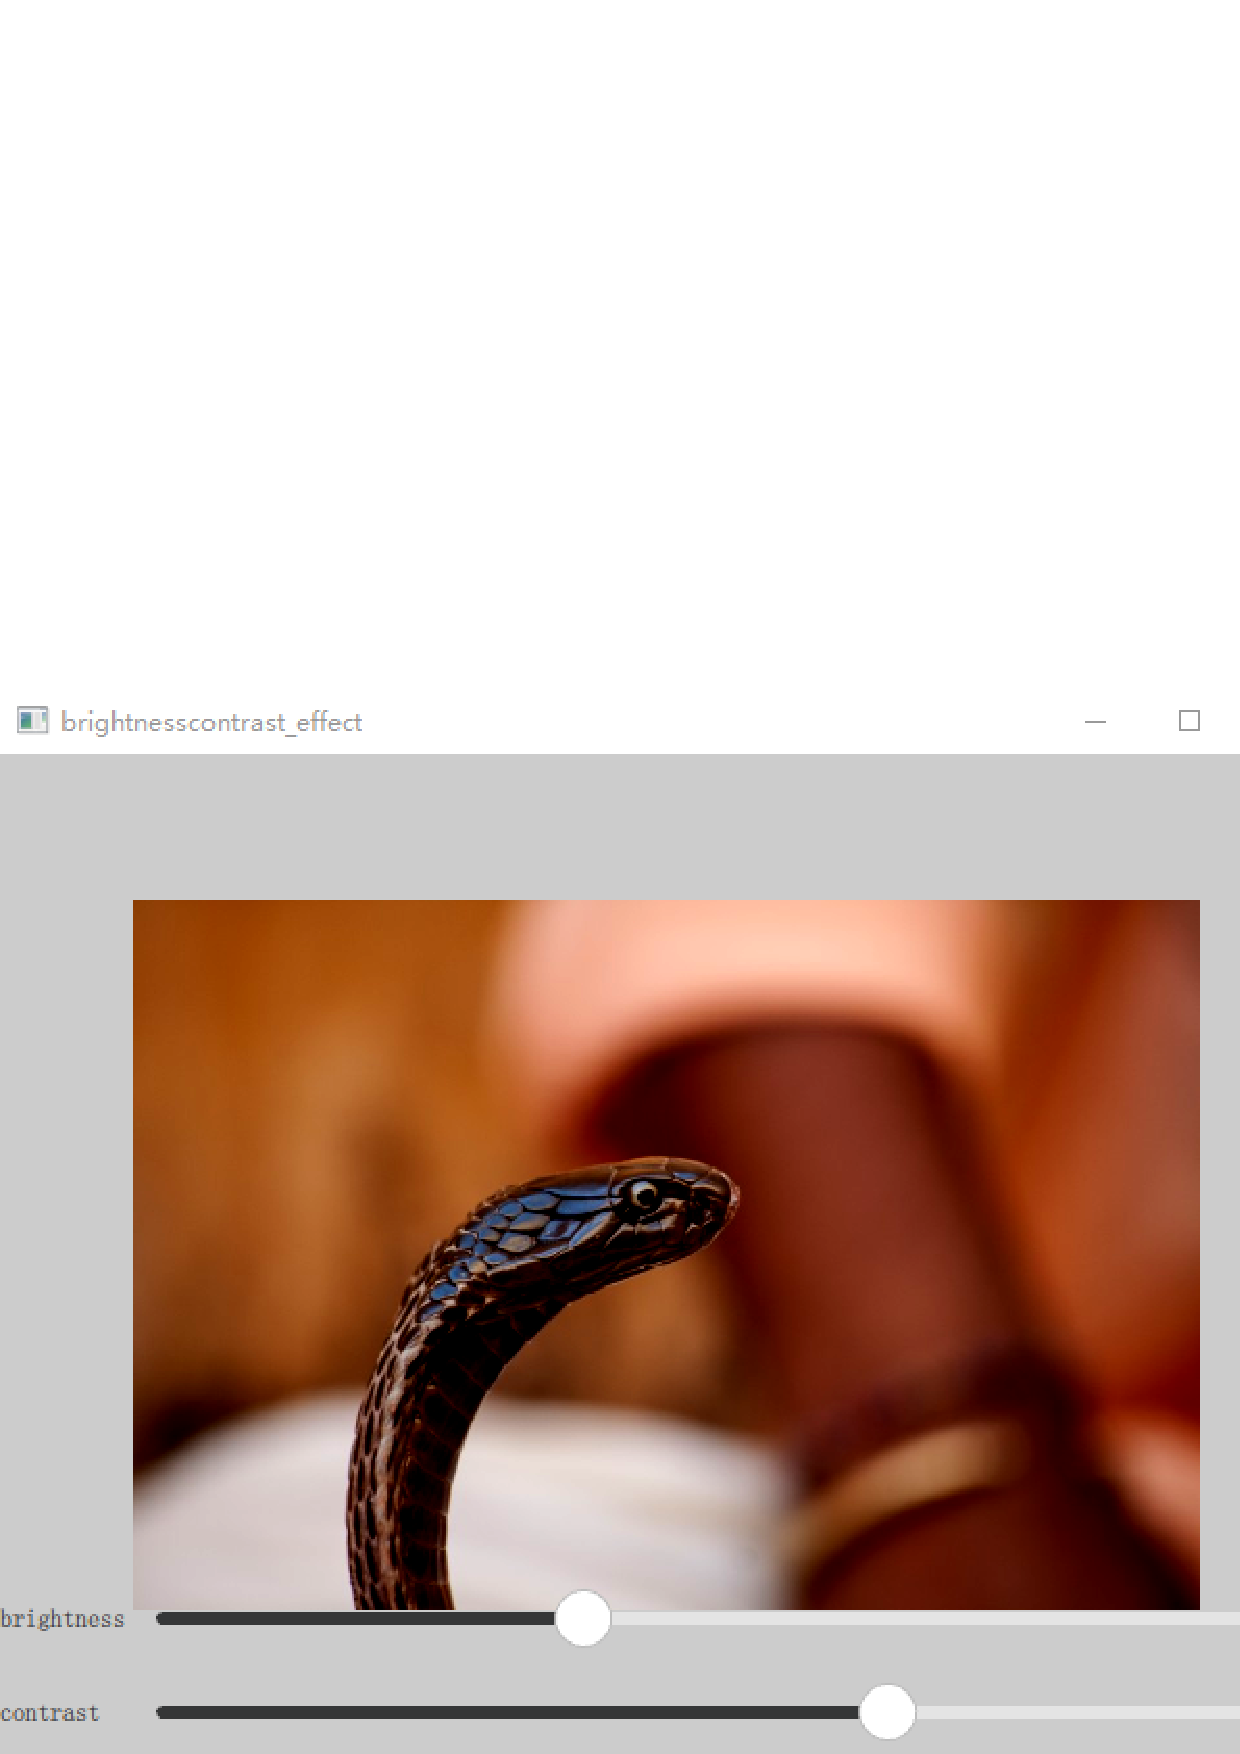
\includegraphics[width=0.95\textwidth]{the_book_image/p000019.pdf}} %图片路径
\caption{BrightnessContrast} %标题
\label{p000019} %索引
\end{figure}
%end图片


%\begin{spacing}{1.0}
\refstepcounter{filesourcenumber}\label{f000053}    %增加源代码编号
\FloatBarrier                                  %强制完成浮动体布局
\begin{thebookfilesourceone}[escapeinside={(*@}{@*)},
caption=GoodLuck,
title=\filesourcenumbernameone \thefilesourcenumber
]
/*brightnesscontrast_effect/main.qml*/
import QtQuick 2.9
import QtGraphicalEffects 1.12

Rectangle {

    id : idRoot
    width: 640;
    height: 480;
    color: Qt.rgba(0.8,0.8,0.8,1);


    Image{
        width: parent.width * 0.8;
        height: parent.height * 0.8;
        anchors.centerIn: parent
        source: "image.jpg"
        visible: false
        fillMode: Image.PreserveAspectFit
        id : idImage
    }

    BrightnessContrast{
        anchors.fill: idImage
        source: idImage
        contrast: idControl.contrastItem.value
        brightness: idControl.brightnessItem.value
    }

    BrightnessContrastControl{
        id:idControl
    }

}(*@\marginpar[\hfill\setlength\fboxsep{2pt}\fbox{\footnotesize{\kaishu\parbox{1em}{\setlength{\baselineskip}{2pt}\filesourcenumbernameone}}\footnotesize{\thefilesourcenumber}}]{\setlength\fboxsep{2pt}\fbox{\footnotesize{\kaishu\parbox{1em}{\setlength{\baselineskip}{2pt}\filesourcenumbernameone}}\footnotesize{\thefilesourcenumber}}}@*)\end{thebookfilesourceone}          %抄录环境
\addtocounter{lstlisting}{-1}   %sub lstlisting counter ...
%\end{spacing}



% ______all_key_words
% the_book_chapter the_book_subsection the_book_subsubsection
% the_book_section the_book_image the_book_table
% the_book_file the_book_tree_file the_book_command_file
% littlelongworld tabbing ref
% figurename tablename filesourcenumbernameone
% treeindexnumbernameone commandnumbernameone footnote
% item itemize comment textbullet
% \hspace*{\parindent}







%使用XeLaTeX编译
%版权所有,翻版必究
%本文件由程序自动生成,任何修改将被覆盖
%2019 年 01 月 23 日





%使用XeLaTeX编译
%版权所有,翻版必究
%本文件由程序自动生成,任何修改将被覆盖
%2019 年 01 月 23 日




\FloatBarrier
\section{
ColorOverlay
}\label{c000015s000004}



未完待续






%使用XeLaTeX编译
%版权所有,翻版必究
%本文件由程序自动生成,任何修改将被覆盖
%2019 年 01 月 23 日





%使用XeLaTeX编译
%版权所有,翻版必究
%本文件由程序自动生成,任何修改将被覆盖
%2019 年 01 月 23 日




\FloatBarrier
\section{
Colorize
}\label{c000015s000005}


%begin图片
\begin{figure}[htb] %浮动体 here and top ...
%there must use marginnote not use marginnote ...
\marginnote{\setlength\fboxsep{2pt}\fbox{\footnotesize{\kaishu\figurename\,}\footnotesize{\ref{p000021}}}}\centering %中心对齐
\includegraphics[width=0.95\textwidth]{../chapter06/colorize_effect/the_app.png} %图片路径
\caption{Colorize} %标题
\label{p000021} %索引
\end{figure}
%end图片


未完待续






%使用XeLaTeX编译
%版权所有,翻版必究
%本文件由程序自动生成,任何修改将被覆盖
%2019 年 01 月 23 日





%使用XeLaTeX编译
%版权所有,翻版必究
%本文件由程序自动生成,任何修改将被覆盖
%2019 年 01 月 23 日




\FloatBarrier
\section{
Desaturate
}\label{c000015s000006}


%begin图片
\begin{figure}[htb] %浮动体 here and top ...
%there must use marginnote not use marginnote ...
\marginnote{\setlength\fboxsep{2pt}\fbox{\footnotesize{\kaishu\figurename\,}\footnotesize{\ref{p000022}}}}\centering %中心对齐
\includegraphics[width=0.95\textwidth]{../chapter06/desaturate_effect/the_app.png} %图片路径
\caption{Desaturate} %标题
\label{p000022} %索引
\end{figure}
%end图片


未完待续






%使用XeLaTeX编译
%版权所有,翻版必究
%本文件由程序自动生成,任何修改将被覆盖
%2019 年 01 月 23 日




\input{chapter06/GammaAdjust.tex}

%使用XeLaTeX编译
%版权所有,翻版必究
%本文件由程序自动生成,任何修改将被覆盖
%2019 年 01 月 23 日




\FloatBarrier
\section{
HueSaturation
}\label{c000015s000008}


%begin图片
\begin{figure}[htb] %浮动体 here and top ...
%there must use marginnote ...
\marginnote{\setlength\fboxsep{2pt}\fbox{\footnotesize{\kaishu\figurename\,}\footnotesize{\ref{p000024}}}}\centering %中心对齐
\includegraphics[width=0.95\textwidth]{../chapter06/huesaturation_effect/the_app.png} %图片路径
\caption{HueSaturation} %标题
\label{p000024} %索引
\end{figure}
%end图片


%\begin{spacing}{1.0}
\refstepcounter{filesourcenumber}\label{f000058}    %增加源代码编号
\FloatBarrier                                  %强制完成浮动体布局
\begin{thebookfilesourceone}[escapeinside={(*@}{@*)},
caption=GoodLuck,
title=\filesourcenumbernameone \thefilesourcenumber
]
/*huesaturation_effect/main.qml*/
import QtQuick 2.9
import QtGraphicalEffects 1.12

Rectangle {
    id : idRoot
    width: 640;
    height: 480;
    color: Qt.rgba(0.8,0.8,0.8,1);

    Image{
        width: parent.width * 0.8;
        height: parent.height * 0.8;
        anchors.centerIn: parent
        source: "image"
        visible: false
        fillMode: Image.PreserveAspectFit
        id : idImage
    }

    HueSaturation{
        anchors.fill: idImage
        source: idImage
        hue : thisControl.hueItem.value
        lightness: thisControl.lightnessItem.value
        saturation: thisControl.saturationItem.value
    }

    HuesaturationControl{
        id : thisControl
    }

}(*@\marginpar[\hfill\setlength\fboxsep{2pt}\fbox{\footnotesize{\kaishu\parbox{1em}{\setlength{\baselineskip}{2pt}\filesourcenumbernameone}}\footnotesize{\thefilesourcenumber}}]{\setlength\fboxsep{2pt}\fbox{\footnotesize{\kaishu\parbox{1em}{\setlength{\baselineskip}{2pt}\filesourcenumbernameone}}\footnotesize{\thefilesourcenumber}}}@*)\end{thebookfilesourceone}          %抄录环境
\addtocounter{lstlisting}{-1}   %sub lstlisting counter ...
%\end{spacing}


未完待续






%使用XeLaTeX编译
%版权所有,翻版必究
%本文件由程序自动生成,任何修改将被覆盖
%2019 年 01 月 23 日




\input{chapter06/LevelAdjust.tex}
\input{chapter06/ConicalGradient.tex}
\input{chapter06/LinearGradient.tex}

%使用XeLaTeX编译
%版权所有,翻版必究
%本文件由程序自动生成,任何修改将被覆盖
%2019 年 01 月 23 日




\FloatBarrier
\section{
RadialGradient
}\label{c000015s000012}


%begin图片
\begin{figure}[htb] %浮动体 here and top ...
%there must use marginnote ...
\marginnote{\setlength\fboxsep{2pt}\fbox{\footnotesize{\kaishu\figurename\,}\footnotesize{\ref{p000028}}}}\centering %中心对齐
\setlength\fboxsep{0pt}\fcolorbox[rgb]{0,0,0}{0.97,0.98,0.99}{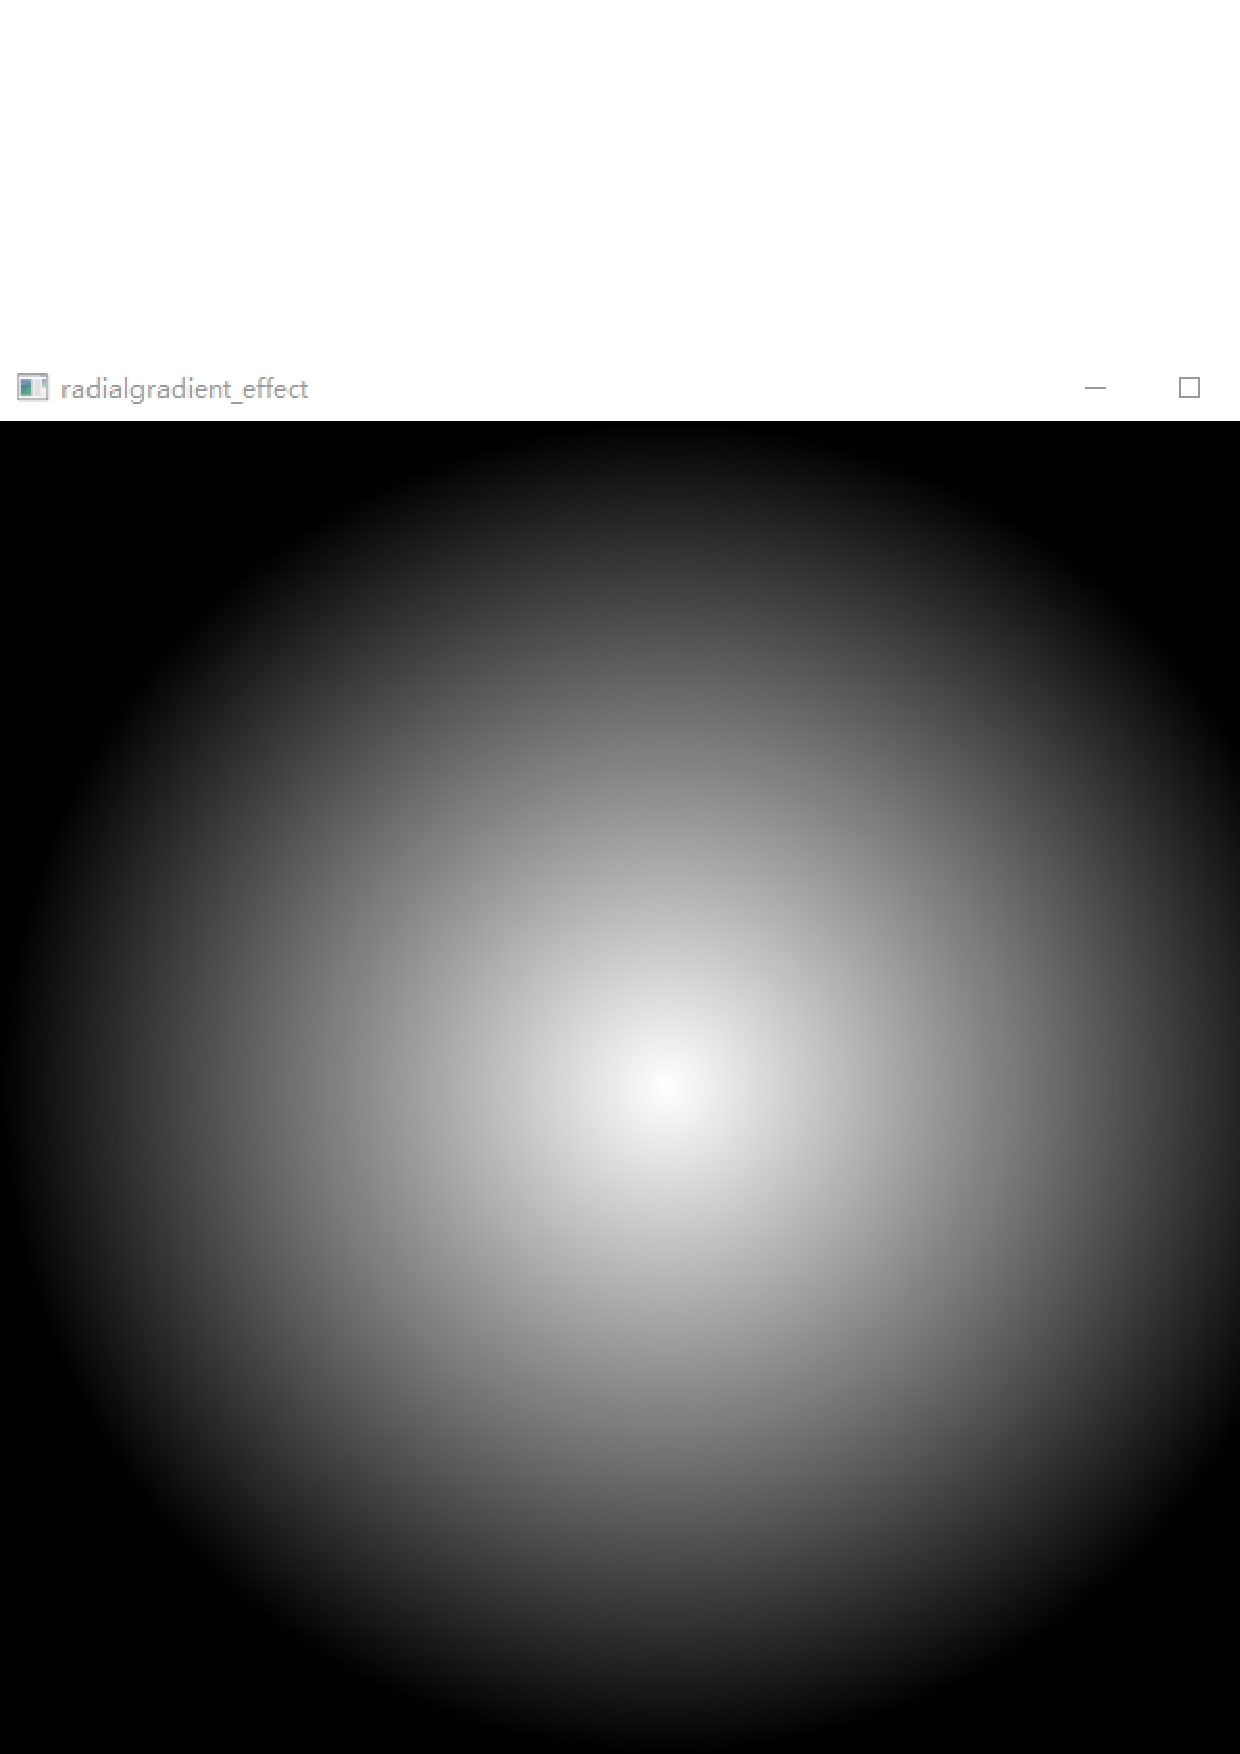
\includegraphics[width=0.95\textwidth]{the_book_image/p000028.pdf}} %图片路径
\caption{RadialGradient} %标题
\label{p000028} %索引
\end{figure}
%end图片


%\begin{spacing}{1.0}
\refstepcounter{filesourcenumber}\label{f000062}    %增加源代码编号
\FloatBarrier                                  %强制完成浮动体布局
\begin{thebookfilesourceone}[escapeinside={(*@}{@*)},
caption=GoodLuck,
title=\filesourcenumbernameone \thefilesourcenumber
]
/*radialgradient_effect/main.qml*/
import QtQuick 2.9
import QtGraphicalEffects 1.12

Rectangle {
    id : idRoot
    width: 640;
    height: 640;
    color: Qt.rgba(0.8,0.8,0.8,1);

    RadialGradient {
        anchors.fill: parent
        gradient: Gradient {
            GradientStop { position: 0.0; color: "white" }
            GradientStop { position: 0.5; color: "black" }
        }
    }

}(*@\marginpar[\hfill\setlength\fboxsep{2pt}\fbox{\footnotesize{\kaishu\parbox{1em}{\setlength{\baselineskip}{2pt}\filesourcenumbernameone}}\footnotesize{\thefilesourcenumber}}]{\setlength\fboxsep{2pt}\fbox{\footnotesize{\kaishu\parbox{1em}{\setlength{\baselineskip}{2pt}\filesourcenumbernameone}}\footnotesize{\thefilesourcenumber}}}@*)\end{thebookfilesourceone}          %抄录环境
\addtocounter{lstlisting}{-1}   %sub lstlisting counter ...
%\end{spacing}


未完待续


% ______all_key_words
% the_book_chapter the_book_subsection the_book_subsubsection
% the_book_section the_book_image the_book_table
% the_book_file the_book_tree_file the_book_command_file
% littlelongworld tabbing ref
% figurename tablename filesourcenumbernameone
% treeindexnumbernameone commandnumbernameone footnote 
% item itemize comment textbullet
% \hspace*{\parindent}







%使用XeLaTeX编译
%版权所有,翻版必究
%本文件由程序自动生成,任何修改将被覆盖
%2019 年 01 月 23 日





%使用XeLaTeX编译
%版权所有,翻版必究
%本文件由程序自动生成,任何修改将被覆盖
%2019 年 01 月 23 日




\FloatBarrier
\section{
Displace
}\label{c000015s000013}


%begin图片
\begin{figure}[htb] %浮动体 here and top ...
%there must use marginnote not use marginnote ...
\marginnote{\setlength\fboxsep{2pt}\fbox{\footnotesize{\kaishu\figurename\,}\footnotesize{\ref{p000029}}}}\centering %中心对齐
\includegraphics[width=0.95\textwidth]{../chapter06/displace_effect/the_app.png} %图片路径
\caption{Displace} %标题
\label{p000029} %索引
\end{figure}
%end图片


未完待续






%使用XeLaTeX编译
%版权所有,翻版必究
%本文件由程序自动生成,任何修改将被覆盖
%2019 年 01 月 23 日




\input{chapter06/DropShadow.tex}
\input{chapter06/InnerShadow.tex}
\input{chapter06/FastBlur.tex}

%使用XeLaTeX编译
%版权所有,翻版必究
%本文件由程序自动生成,任何修改将被覆盖
%2019 年 01 月 23 日




\FloatBarrier
\section{
GaussianBlur
}\label{c000015s000017}


%begin图片
\begin{figure}[htb] %浮动体 here and top ...
%there must use marginnote not use marginnote ...
\marginnote{\setlength\fboxsep{2pt}\fbox{\footnotesize{\kaishu\figurename\,}\footnotesize{\ref{p000033}}}}\centering %中心对齐
\includegraphics[width=0.95\textwidth]{../chapter06/gaussianblur_effect/the_app.png} %图片路径
\caption{GaussianBlur} %标题
\label{p000033} %索引
\end{figure}
%end图片


%\begin{spacing}{1.0}
\refstepcounter{filesourcenumber}\label{f000067}    %增加源代码编号
\FloatBarrier                                  %强制完成浮动体布局
\begin{thebookfilesourceone}[escapeinside={(*@}{@*)},
caption=GoodLuck,
title=\filesourcenumbernameone \thefilesourcenumber
]
/*gaussianblur_effect/main.qml*/
import QtQuick 2.9
import QtGraphicalEffects 1.12

Rectangle {
    id : idRoot
    width: 640;
    height: 480;
    color: Qt.rgba(0.8,0.8,0.8,1);

    Image{
        width: parent.width * 0.8;
        height: parent.height * 0.8;
        anchors.centerIn: parent
        source: "image"
        visible: false
        fillMode: Image.PreserveAspectFit
        id : idImage
    }

    GaussianBlur{
        anchors.fill: idImage
        source: idImage
        radius: 8
        samples: 16
        deviation: idThisControl.deviationItem.value
    }

    GaussianBlurControl{
        id : idThisControl
    }

}(*@\marginpar[\hfill\setlength\fboxsep{2pt}\fbox{\footnotesize{\kaishu\parbox{1em}{\setlength{\baselineskip}{2pt}\filesourcenumbernameone}}\footnotesize{\thefilesourcenumber}}]{\setlength\fboxsep{2pt}\fbox{\footnotesize{\kaishu\parbox{1em}{\setlength{\baselineskip}{2pt}\filesourcenumbernameone}}\footnotesize{\thefilesourcenumber}}}@*)\end{thebookfilesourceone}          %抄录环境
\addtocounter{lstlisting}{-1}   %sub lstlisting counter ...
%\end{spacing}


未完待续






%使用XeLaTeX编译
%版权所有,翻版必究
%本文件由程序自动生成,任何修改将被覆盖
%2019 年 01 月 23 日




\input{chapter06/MaskedBlur.tex}
\input{chapter06/RecursiveBlur.tex}

%使用XeLaTeX编译
%版权所有,翻版必究
%本文件由程序自动生成,任何修改将被覆盖
%2019 年 01 月 23 日




\FloatBarrier
\section{
DirectionalBlur
}\label{c000015s000020}


%begin图片
\begin{figure}[htb] %浮动体 here and top ...
%there must use marginnote ...
\marginnote{\setlength\fboxsep{2pt}\fbox{\footnotesize{\kaishu\figurename\,}\footnotesize{\ref{p000036}}}}\centering %中心对齐
\setlength\fboxsep{0pt}\fcolorbox[rgb]{0,0,0}{0,0,0}{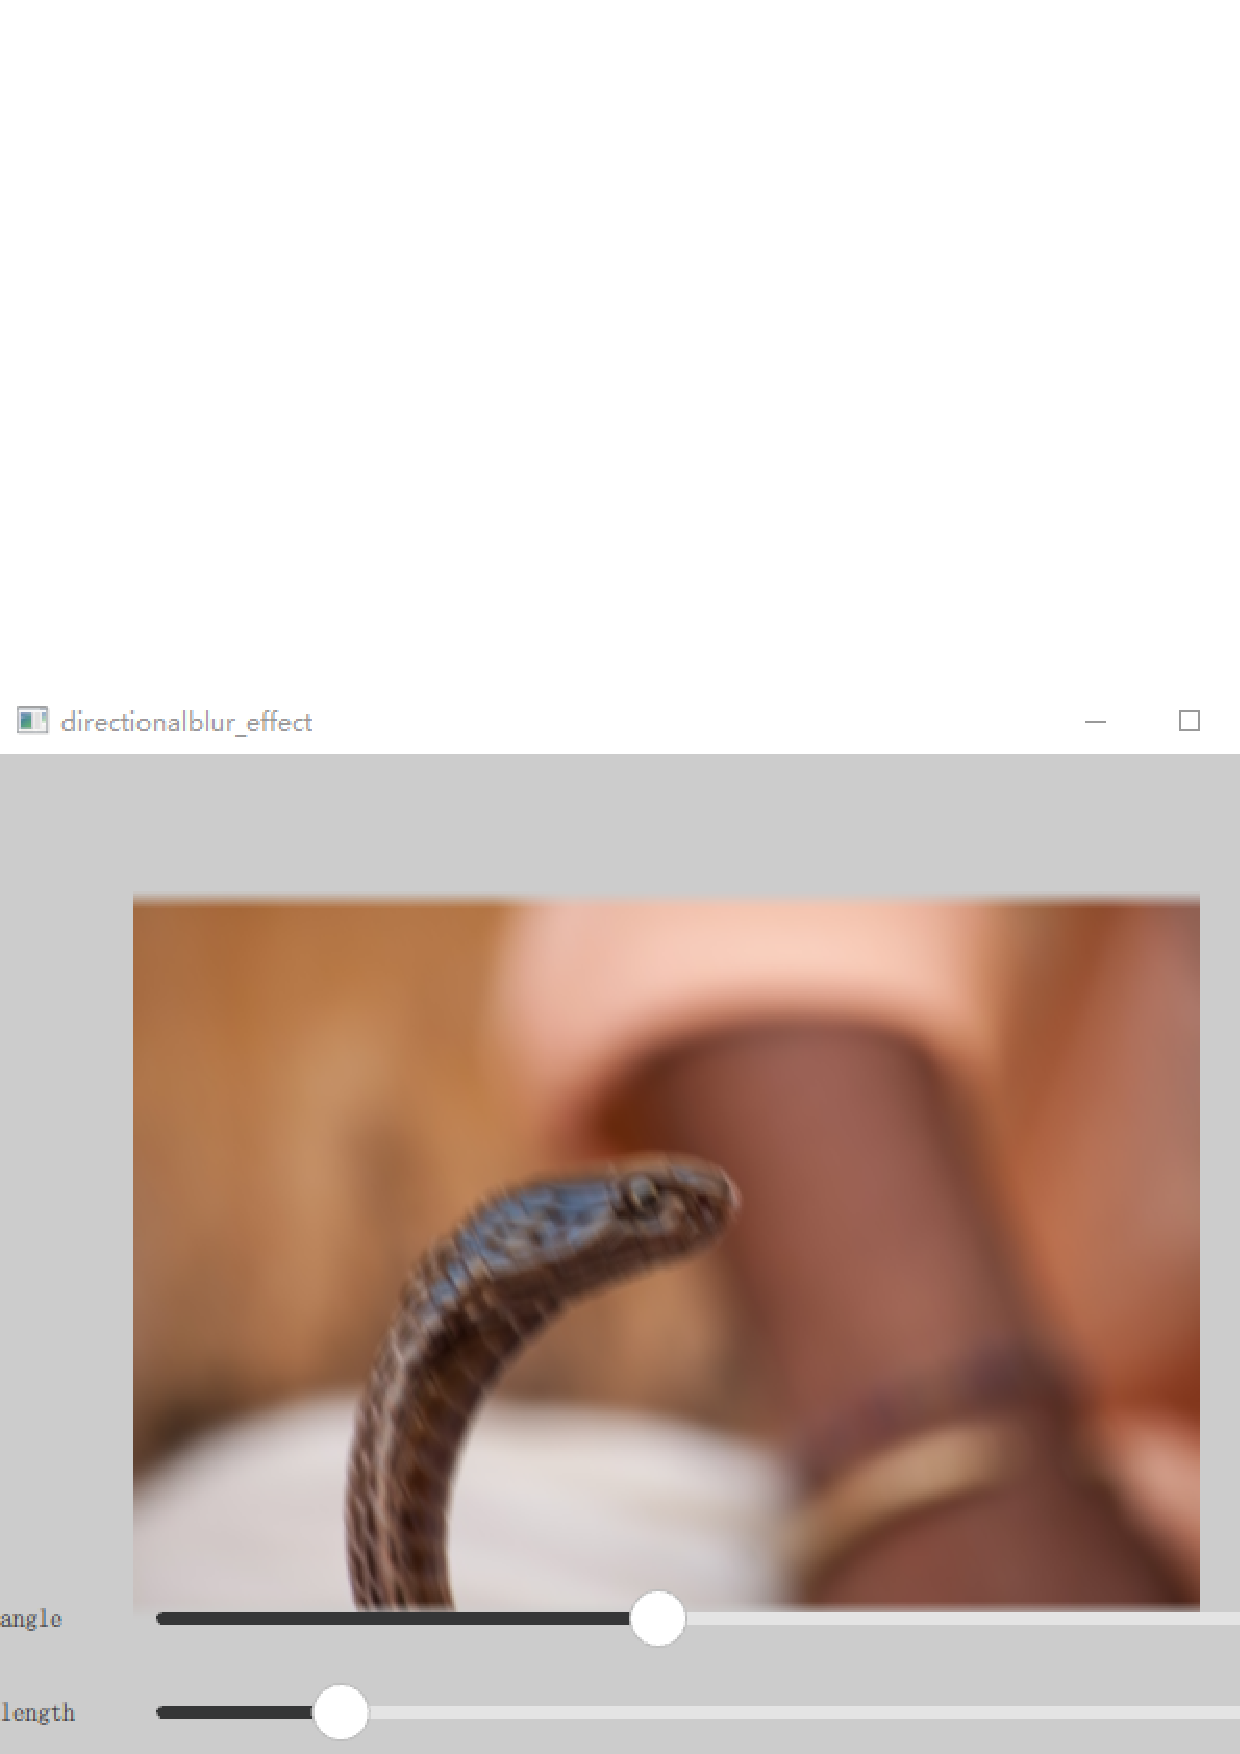
\includegraphics[width=0.95\textwidth]{the_book_image/p000036.pdf}} %图片路径
\caption{DirectionalBlur} %标题
\label{p000036} %索引
\end{figure}
%end图片


%\begin{spacing}{1.0}
\refstepcounter{filesourcenumber}\label{f000070}    %增加源代码编号
\FloatBarrier                                  %强制完成浮动体布局
\begin{thebookfilesourceone}[escapeinside={(*@}{@*)},
caption=GoodLuck,
title=\filesourcenumbernameone \thefilesourcenumber
]
/*directionalblur_effect/main.qml*/
import QtQuick 2.9
import QtGraphicalEffects 1.12

Rectangle {
    id : idRoot
    width: 640;
    height: 480;
    color: Qt.rgba(0.8,0.8,0.8,1);

    Image{
        width: parent.width * 0.8;
        height: parent.height * 0.8;
        anchors.centerIn: parent
        source: "image.jpg"
        visible: false
        fillMode: Image.PreserveAspectFit
        id : idImage
    }

    DirectionalBlur{
        anchors.fill: idImage
        source: idImage
        samples: 64
        length: idThisControl.lengthItem.value
        angle: idThisControl.angleItem.value
        transparentBorder : false
        id:idEffect
    }

    DirectionalblurControl{
        id : idThisControl
        lengthItem.to: idEffect.samples
    }

}(*@\marginpar[\hfill\setlength\fboxsep{2pt}\fbox{\footnotesize{\kaishu\parbox{1em}{\setlength{\baselineskip}{2pt}\filesourcenumbernameone}}\footnotesize{\thefilesourcenumber}}]{\setlength\fboxsep{2pt}\fbox{\footnotesize{\kaishu\parbox{1em}{\setlength{\baselineskip}{2pt}\filesourcenumbernameone}}\footnotesize{\thefilesourcenumber}}}@*)\end{thebookfilesourceone}          %抄录环境
\addtocounter{lstlisting}{-1}   %sub lstlisting counter ...
%\end{spacing}


未完待续






%使用XeLaTeX编译
%版权所有,翻版必究
%本文件由程序自动生成,任何修改将被覆盖
%2019 年 01 月 23 日




\input{chapter06/RadialBlur.tex}

%使用XeLaTeX编译
%版权所有,翻版必究
%本文件由程序自动生成,任何修改将被覆盖
%2019 年 01 月 23 日




\FloatBarrier
\section{
ZoomBlur
}\label{c000015s000022}


%begin图片
\begin{figure}[htb] %浮动体 here and top ...
%there must use marginnote not use marginnote ...
\marginnote{\setlength\fboxsep{2pt}\fbox{\footnotesize{\kaishu\figurename\,}\footnotesize{\ref{p000038}}}}\centering %中心对齐
\includegraphics[width=0.95\textwidth]{../chapter06/zoomblur_effect/the_app.png} %图片路径
\caption{ZoomBlur} %标题
\label{p000038} %索引
\end{figure}
%end图片


未完待续






%使用XeLaTeX编译
%版权所有,翻版必究
%本文件由程序自动生成,任何修改将被覆盖
%2019 年 01 月 23 日




\input{chapter06/Glow.tex}

%使用XeLaTeX编译
%版权所有,翻版必究
%本文件由程序自动生成,任何修改将被覆盖
%2019 年 01 月 23 日




\FloatBarrier
\section{
RectangularGlow
}\label{c000015s000024}


%begin图片
\begin{figure}[htb] %浮动体 here and top ...
%there must use marginnote not use marginnote ...
\marginnote{\setlength\fboxsep{2pt}\fbox{\footnotesize{\kaishu\figurename\,}\footnotesize{\ref{p000040}}}}\centering %中心对齐
\includegraphics[width=0.95\textwidth]{../chapter06/rectangularglow_effect/the_app.png} %图片路径
\caption{RectangularGlow} %标题
\label{p000040} %索引
\end{figure}
%end图片


未完待续






%使用XeLaTeX编译
%版权所有,翻版必究
%本文件由程序自动生成,任何修改将被覆盖
%2019 年 01 月 23 日




\input{chapter06/OpacityMask.tex}
\input{chapter06/ThresholdMask.tex}




% ______all_key_words
% the_book_chapter the_book_subsection the_book_subsubsection
% the_book_section the_book_image the_book_table
% the_book_file the_book_tree_file the_book_command_file
% littlelongworld tabbing ref
% figurename tablename filesourcenumbernameone
% treeindexnumbernameone commandnumbernameone footnote 
% item itemize comment textbullet
% \hspace*{\parindent}







%使用XeLaTeX编译
%版权所有,翻版必究
%本文件由程序自动生成,任何修改将被覆盖
%2019 年 01 月 23 日



   %第六章
%使用xelatex编译
%版权所有,翻版必究
%本文件由程序自动生成,任何修改将被覆盖





\cleardoublepage
\chapter{
多媒体
}


















%使用xelatex编译
%版权所有,翻版必究
%本文件由程序自动生成,任何修改将被覆盖



   %第七章
\input{chapter08/chapter08.tex}   %第八章

%使用XeLaTeX编译
%版权所有,翻版必究
%本文件由程序自动生成,任何修改将被覆盖
%2019 年 01 月 23 日




%\FloatBarrier
\cleardoublepage
\chapter{
控件
}\label{c000018}



















%使用XeLaTeX编译
%版权所有,翻版必究
%本文件由程序自动生成,任何修改将被覆盖
%2019 年 01 月 23 日



   %第九章

%使用XeLaTeX编译
%版权所有,翻版必究
%本文件由程序自动生成,任何修改将被覆盖
%2019 年 01 月 23 日




%\FloatBarrier
\cleardoublepage
\chapter{
模型视图
}\label{c000019}


Qt Widgets中的模型视图非常难用。

在Qt Widgets中的模型视图
架构中,每一个单独的项不是
一个单独的QWidget。
而是通过QPainter进行绘制,
并通过一些函数响应鼠标键盘事件。

这就造成了如果读者想
实现一些复杂的动态效果就
不得不自己实现一个超级复杂
的状态机系统。

而在Qt Quick中一切可视元素都是一致的。

视图是QQuickItem的子类,
视图中的每一项也是QQuickItem的子类。
在Qt Quick体系中一切都是对象!

读者可以使用Qt Quick的模型视图架构,
将数据与渲染和控制完全分离。
而且,
这种实现是极其高效的,
即使模型拥有高达数亿元素。
Qt Quick的模型视图架构也可以快速
布局并迅速渲染。











%使用XeLaTeX编译
%版权所有,翻版必究
%本文件由程序自动生成,任何修改将被覆盖
%2019 年 01 月 23 日



   %第十章

\backmatter
%%%%%%%%%%%%%%%%%%%%%%%%%%%%%%%%%%%%%%%%%%%%%%%%%%%%%%%%%%%%%%%%%%%%%%%%%%%%%

\end{document}

%http://www.ctex.org/documents/latex/graphics/node2.html











%使用xelatex编译
%版权所有,翻版必究
%本文件由程序自动生成,任何修改将被覆盖
%2019 年 01 月 09 日



